\documentclass[twoside]{book}

% Packages required by doxygen
\usepackage{fixltx2e}
\usepackage{calc}
\usepackage{doxygen}
\usepackage[export]{adjustbox} % also loads graphicx
\usepackage{graphicx}
\usepackage[utf8]{inputenc}
\usepackage{makeidx}
\usepackage{multicol}
\usepackage{multirow}
\PassOptionsToPackage{warn}{textcomp}
\usepackage{textcomp}
\usepackage[nointegrals]{wasysym}
\usepackage[table]{xcolor}

% Font selection
\usepackage[T1]{fontenc}
\usepackage[scaled=.90]{helvet}
\usepackage{courier}
\usepackage{amssymb}
\usepackage{sectsty}
\renewcommand{\familydefault}{\sfdefault}
\allsectionsfont{%
  \fontseries{bc}\selectfont%
  \color{darkgray}%
}
\renewcommand{\DoxyLabelFont}{%
  \fontseries{bc}\selectfont%
  \color{darkgray}%
}
\newcommand{\+}{\discretionary{\mbox{\scriptsize$\hookleftarrow$}}{}{}}

% Page & text layout
\usepackage{geometry}
\geometry{%
  a4paper,%
  top=2.5cm,%
  bottom=2.5cm,%
  left=2.5cm,%
  right=2.5cm%
}
\tolerance=750
\hfuzz=15pt
\hbadness=750
\setlength{\emergencystretch}{15pt}
\setlength{\parindent}{0cm}
\setlength{\parskip}{3ex plus 2ex minus 2ex}
\makeatletter
\renewcommand{\paragraph}{%
  \@startsection{paragraph}{4}{0ex}{-1.0ex}{1.0ex}{%
    \normalfont\normalsize\bfseries\SS@parafont%
  }%
}
\renewcommand{\subparagraph}{%
  \@startsection{subparagraph}{5}{0ex}{-1.0ex}{1.0ex}{%
    \normalfont\normalsize\bfseries\SS@subparafont%
  }%
}
\makeatother

% Headers & footers
\usepackage{fancyhdr}
\pagestyle{fancyplain}
\fancyhead[LE]{\fancyplain{}{\bfseries\thepage}}
\fancyhead[CE]{\fancyplain{}{}}
\fancyhead[RE]{\fancyplain{}{\bfseries\leftmark}}
\fancyhead[LO]{\fancyplain{}{\bfseries\rightmark}}
\fancyhead[CO]{\fancyplain{}{}}
\fancyhead[RO]{\fancyplain{}{\bfseries\thepage}}
\fancyfoot[LE]{\fancyplain{}{}}
\fancyfoot[CE]{\fancyplain{}{}}
\fancyfoot[RE]{\fancyplain{}{\bfseries\scriptsize Generated by Doxygen }}
\fancyfoot[LO]{\fancyplain{}{\bfseries\scriptsize Generated by Doxygen }}
\fancyfoot[CO]{\fancyplain{}{}}
\fancyfoot[RO]{\fancyplain{}{}}
\renewcommand{\footrulewidth}{0.4pt}
\renewcommand{\chaptermark}[1]{%
  \markboth{#1}{}%
}
\renewcommand{\sectionmark}[1]{%
  \markright{\thesection\ #1}%
}

% Indices & bibliography
\usepackage{natbib}
\usepackage[titles]{tocloft}
\setcounter{tocdepth}{3}
\setcounter{secnumdepth}{5}
\makeindex

% Hyperlinks (required, but should be loaded last)
\usepackage{ifpdf}
\ifpdf
  \usepackage[pdftex,pagebackref=true]{hyperref}
\else
  \usepackage[ps2pdf,pagebackref=true]{hyperref}
\fi
\hypersetup{%
  colorlinks=true,%
  linkcolor=blue,%
  citecolor=blue,%
  unicode%
}

% Custom commands
\newcommand{\clearemptydoublepage}{%
  \newpage{\pagestyle{empty}\cleardoublepage}%
}

\usepackage{caption}
\captionsetup{labelsep=space,justification=centering,font={bf},singlelinecheck=off,skip=4pt,position=top}

%===== C O N T E N T S =====

\begin{document}

% Titlepage & ToC
\hypersetup{pageanchor=false,
             bookmarksnumbered=true,
             pdfencoding=unicode
            }
\pagenumbering{alph}
\begin{titlepage}
\vspace*{7cm}
\begin{center}%
{\Large A\+PO Light Control }\\
\vspace*{1cm}
{\large Generated by Doxygen 1.8.14}\\
\end{center}
\end{titlepage}
\clearemptydoublepage
\pagenumbering{roman}
\tableofcontents
\clearemptydoublepage
\pagenumbering{arabic}
\hypersetup{pageanchor=true}

%--- Begin generated contents ---
\chapter{Module Index}
\section{Modules}
Here is a list of all modules\+:\begin{DoxyCompactList}
\item \contentsline{section}{Title for records module}{\pageref{group__Colours}}{}
\end{DoxyCompactList}

\chapter{Namespace Index}
\section{Namespace List}
Here is a list of all documented namespaces with brief descriptions\+:\begin{DoxyCompactList}
\item\contentsline{section}{\mbox{\hyperlink{namespaceColour}{Colour}} \\*Anything related to handling colours }{\pageref{namespaceColour}}{}
\item\contentsline{section}{\mbox{\hyperlink{namespaceEngine}{Engine}} \\*Namesapce representing the entry point of the application }{\pageref{namespaceEngine}}{}
\item\contentsline{section}{\mbox{\hyperlink{namespaceIOTools}{I\+O\+Tools}} \\*Tools connected to IO }{\pageref{namespaceIOTools}}{}
\item\contentsline{section}{\mbox{\hyperlink{namespaceLedController}{Led\+Controller}} \\*Namespace that handles L\+E\+Ds }{\pageref{namespaceLedController}}{}
\end{DoxyCompactList}

\chapter{Hierarchical Index}
\section{Class Hierarchy}
This inheritance list is sorted roughly, but not completely, alphabetically\+:\begin{DoxyCompactList}
\item \contentsline{section}{Control\+Message\+Queue\+:\+:Control\+Message\+Info}{\pageref{structControlMessageQueue_1_1ControlMessageInfo}}{}
\item \contentsline{section}{Control\+Message\+Queue}{\pageref{classControlMessageQueue}}{}
\item \contentsline{section}{Device\+Input}{\pageref{classDeviceInput}}{}
\item \contentsline{section}{Display}{\pageref{classDisplay}}{}
\item \contentsline{section}{font\+\_\+descriptor\+\_\+t}{\pageref{structfont__descriptor__t}}{}
\item \contentsline{section}{Light\+Unit}{\pageref{classLightUnit}}{}
\item \contentsline{section}{Mapper}{\pageref{classMapper}}{}
\item \contentsline{section}{Network\+Handler\+:\+:Message}{\pageref{structNetworkHandler_1_1Message}}{}
\begin{DoxyCompactList}
\item \contentsline{section}{Network\+Handler\+:\+:Broadcast\+Message}{\pageref{structNetworkHandler_1_1BroadcastMessage}}{}
\item \contentsline{section}{Network\+Handler\+:\+:Control\+Message}{\pageref{structNetworkHandler_1_1ControlMessage}}{}
\end{DoxyCompactList}
\item \contentsline{section}{Network\+Handler}{\pageref{classNetworkHandler}}{}
\item \contentsline{section}{Network\+Handler\+:\+:Recieved\+Message}{\pageref{structNetworkHandler_1_1RecievedMessage}}{}
\item \contentsline{section}{R\+W\+Mutex}{\pageref{classRWMutex}}{}
\item \contentsline{section}{Screen}{\pageref{classScreen}}{}
\begin{DoxyCompactList}
\item \contentsline{section}{List\+Screen}{\pageref{classListScreen}}{}
\item \contentsline{section}{Nyan\+Screen}{\pageref{classNyanScreen}}{}
\item \contentsline{section}{Unit\+Screen}{\pageref{classUnitScreen}}{}
\end{DoxyCompactList}
\end{DoxyCompactList}

\chapter{Class Index}
\section{Class List}
Here are the classes, structs, unions and interfaces with brief descriptions\+:\begin{DoxyCompactList}
\item\contentsline{section}{\mbox{\hyperlink{structNetworkHandler_1_1BroadcastMessage}{Network\+Handler\+::\+Broadcast\+Message}} \\*Broadcast message. Type 0 }{\pageref{structNetworkHandler_1_1BroadcastMessage}}{}
\item\contentsline{section}{\mbox{\hyperlink{classScreen_1_1ColorSquareLineElement}{Screen\+::\+Color\+Square\+Line\+Element}} \\*Color square }{\pageref{classScreen_1_1ColorSquareLineElement}}{}
\item\contentsline{section}{\mbox{\hyperlink{structNetworkHandler_1_1ControlMessage}{Network\+Handler\+::\+Control\+Message}} \\*Control message. Types 1 and 2 }{\pageref{structNetworkHandler_1_1ControlMessage}}{}
\item\contentsline{section}{\mbox{\hyperlink{structControlMessageQueue_1_1ControlMessageInfo}{Control\+Message\+Queue\+::\+Control\+Message\+Info}} \\*Element of the \mbox{\hyperlink{classControlMessageQueue}{Control\+Message\+Queue}} }{\pageref{structControlMessageQueue_1_1ControlMessageInfo}}{}
\item\contentsline{section}{\mbox{\hyperlink{classControlMessageQueue}{Control\+Message\+Queue}} \\*Thread-\/safe F\+I\+FO queue for control messages }{\pageref{classControlMessageQueue}}{}
\item\contentsline{section}{\mbox{\hyperlink{classDeviceInput}{Device\+Input}} \\*Handler device input }{\pageref{classDeviceInput}}{}
\item\contentsline{section}{\mbox{\hyperlink{classDisplay}{Display}} \\*A class that handles the (one-\/way) interaction with the device display and provides methods for rendering shapes, text, and other }{\pageref{classDisplay}}{}
\item\contentsline{section}{\mbox{\hyperlink{structfont__descriptor__t}{font\+\_\+descriptor\+\_\+t}} \\*Bitmap font struct }{\pageref{structfont__descriptor__t}}{}
\item\contentsline{section}{\mbox{\hyperlink{classScreen_1_1IconLineElement}{Screen\+::\+Icon\+Line\+Element}} \\*Scaled icon }{\pageref{classScreen_1_1IconLineElement}}{}
\item\contentsline{section}{\mbox{\hyperlink{classLightUnit}{Light\+Unit}} \\*A class representing a light unit }{\pageref{classLightUnit}}{}
\item\contentsline{section}{\mbox{\hyperlink{classScreen_1_1LineElement}{Screen\+::\+Line\+Element}} \\*Line element base class }{\pageref{classScreen_1_1LineElement}}{}
\item\contentsline{section}{\mbox{\hyperlink{classListScreen}{List\+Screen}} \\*List screen }{\pageref{classListScreen}}{}
\item\contentsline{section}{\mbox{\hyperlink{classMapper}{Mapper}} \\*A class that handles the mapping of peripheral physical regions to virtual addresses }{\pageref{classMapper}}{}
\item\contentsline{section}{\mbox{\hyperlink{structNetworkHandler_1_1Message}{Network\+Handler\+::\+Message}} \\*Base message struct }{\pageref{structNetworkHandler_1_1Message}}{}
\item\contentsline{section}{\mbox{\hyperlink{classNetworkHandler}{Network\+Handler}} \\*Class that handles all network communication }{\pageref{classNetworkHandler}}{}
\item\contentsline{section}{\mbox{\hyperlink{structNetworkHandler_1_1RecievedMessage}{Network\+Handler\+::\+Recieved\+Message}} \\*Struct that represents a recieved message }{\pageref{structNetworkHandler_1_1RecievedMessage}}{}
\item\contentsline{section}{\mbox{\hyperlink{classRWMutex}{R\+W\+Mutex}} \\*Read/\+Write mutex class }{\pageref{classRWMutex}}{}
\item\contentsline{section}{\mbox{\hyperlink{classScreen}{Screen}} \\*Class representing one screen }{\pageref{classScreen}}{}
\item\contentsline{section}{\mbox{\hyperlink{classScreen_1_1SpaceLineElement}{Screen\+::\+Space\+Line\+Element}} \\*Empty space }{\pageref{classScreen_1_1SpaceLineElement}}{}
\item\contentsline{section}{\mbox{\hyperlink{classScreen_1_1TextLineElement}{Screen\+::\+Text\+Line\+Element}} \\*Text }{\pageref{classScreen_1_1TextLineElement}}{}
\item\contentsline{section}{\mbox{\hyperlink{classThemeScreen}{Theme\+Screen}} \\*Theme screen }{\pageref{classThemeScreen}}{}
\item\contentsline{section}{\mbox{\hyperlink{classUnitScreen}{Unit\+Screen}} \\*Unit screen }{\pageref{classUnitScreen}}{}
\end{DoxyCompactList}

\chapter{Module Documentation}
\hypertarget{group__screens}{}\section{Screens}
\label{group__screens}\index{Screens@{Screens}}
\subsection*{Classes}
\begin{DoxyCompactItemize}
\item 
class \mbox{\hyperlink{classListScreen}{List\+Screen}}
\begin{DoxyCompactList}\small\item\em Unit screen. \end{DoxyCompactList}\item 
class \mbox{\hyperlink{classNyanScreen}{Nyan\+Screen}}
\begin{DoxyCompactList}\small\item\em Meow. \end{DoxyCompactList}\item 
class \mbox{\hyperlink{classScreen}{Screen}}
\begin{DoxyCompactList}\small\item\em Class representing one screen. \end{DoxyCompactList}\item 
class \mbox{\hyperlink{classUnitScreen}{Unit\+Screen}}
\begin{DoxyCompactList}\small\item\em Unit screen. \end{DoxyCompactList}\end{DoxyCompactItemize}


\subsection{Detailed Description}

\chapter{Namespace Documentation}
\hypertarget{namespaceColour}{}\section{Colour Namespace Reference}
\label{namespaceColour}\index{Colour@{Colour}}


Anything related to handling colours.  


\subsection*{Enumerations}
\begin{DoxyCompactItemize}
\item 
\mbox{\Hypertarget{namespaceColour_a7eacc5e4e794b134ef740aa5426df245}\label{namespaceColour_a7eacc5e4e794b134ef740aa5426df245}} 
enum \{ \newline
{\bfseries B\+L\+A\+CK} = 0, 
{\bfseries W\+H\+I\+TE} = 0x\+F\+F\+FF, 
{\bfseries R\+ED} = 0x\+F800, 
{\bfseries O\+R\+A\+N\+GE} = 0x\+F\+C00, 
\newline
{\bfseries Y\+E\+L\+L\+OW} = 0x\+F\+F80, 
{\bfseries L\+I\+ME} = 0x\+B7\+E0, 
{\bfseries G\+R\+E\+EN} = 0x4\+F\+E0, 
{\bfseries D\+A\+R\+K\+\_\+\+G\+R\+E\+EN} = 0x4\+D24, 
\newline
{\bfseries B\+L\+UE} = 0x051F, 
{\bfseries P\+U\+R\+P\+LE} = 0x881F, 
{\bfseries B\+R\+O\+WN} = 0x9260, 
{\bfseries D\+A\+R\+K\+\_\+\+B\+L\+UE} = 0x08\+CB, 
\newline
{\bfseries T\+U\+R\+U\+O\+I\+SE} = 0x6694, 
{\bfseries U\+G\+LY} = 0x\+E\+C1A, 
{\bfseries W\+E\+I\+R\+D\+\_\+\+R\+ED} = 0x\+A165, 
{\bfseries D\+A\+R\+K\+\_\+\+G\+R\+EY} = 0x2945, 
\newline
{\bfseries L\+I\+G\+H\+T\+\_\+\+G\+R\+EY} = 0x\+D69A, 
{\bfseries A\+L\+M\+O\+S\+T\+\_\+\+G\+O\+LD} = 0x\+F\+E03
 \}
\end{DoxyCompactItemize}
\subsection*{Functions}
\begin{DoxyCompactItemize}
\item 
uint8\+\_\+t \mbox{\hyperlink{namespaceColour_abad9ffef17d0d47b94a80a834e3b061e}{getR}} (uint32\+\_\+t rgb)
\begin{DoxyCompactList}\small\item\em Extracts the red component from R\+G\+B888. \end{DoxyCompactList}\item 
uint8\+\_\+t \mbox{\hyperlink{namespaceColour_afe62e2366d29eab29349e53694cf04c2}{getG}} (uint32\+\_\+t rgb)
\begin{DoxyCompactList}\small\item\em Extracts the green component from R\+G\+B888. \end{DoxyCompactList}\item 
uint8\+\_\+t \mbox{\hyperlink{namespaceColour_a217843f90fd11c5632683125e19bef08}{getB}} (uint32\+\_\+t rgb)
\begin{DoxyCompactList}\small\item\em Extracts the blue component from R\+G\+B888. \end{DoxyCompactList}\item 
uint32\+\_\+t \mbox{\hyperlink{namespaceColour_aafcc8ab12acc526fa93bee12b961edab}{setR}} (uint32\+\_\+t value, uint8\+\_\+t new\+Value)
\begin{DoxyCompactList}\small\item\em Sets the red component of R\+G\+B888. \end{DoxyCompactList}\item 
uint32\+\_\+t \mbox{\hyperlink{namespaceColour_a059504956471e6a07df579f59cec6e22}{setG}} (uint32\+\_\+t value, uint8\+\_\+t new\+Value)
\begin{DoxyCompactList}\small\item\em Sets the green component of R\+G\+B888. \end{DoxyCompactList}\item 
uint32\+\_\+t \mbox{\hyperlink{namespaceColour_a0b181bcc3bc52f87504d8f1cf3d0289a}{setB}} (uint32\+\_\+t value, uint8\+\_\+t new\+Value)
\begin{DoxyCompactList}\small\item\em Sets the blue component of R\+G\+B888. \end{DoxyCompactList}\item 
uint32\+\_\+t \mbox{\hyperlink{namespaceColour_ad2740cc3e6b9f1d65d6cfe085ec2f1bf}{changeR}} (uint32\+\_\+t value, int16\+\_\+t change)
\begin{DoxyCompactList}\small\item\em Changes the red component of R\+G\+B888. \end{DoxyCompactList}\item 
uint32\+\_\+t \mbox{\hyperlink{namespaceColour_a944d058dabcf1f24a5093a04656efc60}{changeG}} (uint32\+\_\+t value, int16\+\_\+t change)
\begin{DoxyCompactList}\small\item\em Changes the green component of R\+G\+B888. \end{DoxyCompactList}\item 
uint32\+\_\+t \mbox{\hyperlink{namespaceColour_a8e854e6a656f9d7c53dbd46eccba1816}{changeB}} (uint32\+\_\+t value, int16\+\_\+t change)
\begin{DoxyCompactList}\small\item\em Changes the blue component of R\+G\+B888. \end{DoxyCompactList}\item 
uint32\+\_\+t \mbox{\hyperlink{namespaceColour_a2ee4192ca3c1535351e57f223e5fb65d}{from\+R\+GB}} (uint8\+\_\+t r, uint8\+\_\+t g, uint8\+\_\+t b)
\begin{DoxyCompactList}\small\item\em Creates an R\+G\+B888 colour from its separate components. \end{DoxyCompactList}\item 
std\+::string \mbox{\hyperlink{namespaceColour_a317cf8c55a2ec6a9315b50079703ac8f}{to\+R\+G\+B\+String}} (uint32\+\_\+t rgb)
\begin{DoxyCompactList}\small\item\em Creates an rgb string representation of the colour. \end{DoxyCompactList}\item 
std\+::string \mbox{\hyperlink{namespaceColour_a2289444135d7196963b284cdd7f13fff}{to\+Hex\+String}} (uint32\+\_\+t rgb)
\begin{DoxyCompactList}\small\item\em Creates a hex string representation of the colour. \end{DoxyCompactList}\item 
uint16\+\_\+t \mbox{\hyperlink{namespaceColour_a5311fafb2011e62db5d600badee72ee9}{rgb888to565}} (uint32\+\_\+t rgb888)
\begin{DoxyCompactList}\small\item\em Converts an R\+G\+B888 colour to an R\+G\+B565 colour. \end{DoxyCompactList}\item 
uint32\+\_\+t \mbox{\hyperlink{namespaceColour_aa7b3de65f5d56d88b13863de9aa5641a}{rgb565to888}} (uint16\+\_\+t rgb565)
\begin{DoxyCompactList}\small\item\em Converts an R\+G\+B565 colour to an R\+G\+B888 colour. \end{DoxyCompactList}\end{DoxyCompactItemize}


\subsection{Detailed Description}
Anything related to handling colours. 

\subsection{Function Documentation}
\mbox{\Hypertarget{namespaceColour_a8e854e6a656f9d7c53dbd46eccba1816}\label{namespaceColour_a8e854e6a656f9d7c53dbd46eccba1816}} 
\index{Colour@{Colour}!changeB@{changeB}}
\index{changeB@{changeB}!Colour@{Colour}}
\subsubsection{\texorpdfstring{change\+B()}{changeB()}}
{\footnotesize\ttfamily uint32\+\_\+t Colour\+::changeB (\begin{DoxyParamCaption}\item[{uint32\+\_\+t}]{value,  }\item[{int16\+\_\+t}]{change }\end{DoxyParamCaption})}



Changes the blue component of R\+G\+B888. 


\begin{DoxyParams}{Parameters}
{\em value} & The R\+G\+B888 colour to be changed. \\
\hline
{\em change} & The change in the blue component. \\
\hline
\end{DoxyParams}
\mbox{\Hypertarget{namespaceColour_a944d058dabcf1f24a5093a04656efc60}\label{namespaceColour_a944d058dabcf1f24a5093a04656efc60}} 
\index{Colour@{Colour}!changeG@{changeG}}
\index{changeG@{changeG}!Colour@{Colour}}
\subsubsection{\texorpdfstring{change\+G()}{changeG()}}
{\footnotesize\ttfamily uint32\+\_\+t Colour\+::changeG (\begin{DoxyParamCaption}\item[{uint32\+\_\+t}]{value,  }\item[{int16\+\_\+t}]{change }\end{DoxyParamCaption})}



Changes the green component of R\+G\+B888. 


\begin{DoxyParams}{Parameters}
{\em value} & The R\+G\+B888 colour to be changed. \\
\hline
{\em change} & The change in the green component. \\
\hline
\end{DoxyParams}
\mbox{\Hypertarget{namespaceColour_ad2740cc3e6b9f1d65d6cfe085ec2f1bf}\label{namespaceColour_ad2740cc3e6b9f1d65d6cfe085ec2f1bf}} 
\index{Colour@{Colour}!changeR@{changeR}}
\index{changeR@{changeR}!Colour@{Colour}}
\subsubsection{\texorpdfstring{change\+R()}{changeR()}}
{\footnotesize\ttfamily uint32\+\_\+t Colour\+::changeR (\begin{DoxyParamCaption}\item[{uint32\+\_\+t}]{value,  }\item[{int16\+\_\+t}]{change }\end{DoxyParamCaption})}



Changes the red component of R\+G\+B888. 


\begin{DoxyParams}{Parameters}
{\em value} & The R\+G\+B888 colour to be changed. \\
\hline
{\em change} & The change of the red component. \\
\hline
\end{DoxyParams}
\mbox{\Hypertarget{namespaceColour_a2ee4192ca3c1535351e57f223e5fb65d}\label{namespaceColour_a2ee4192ca3c1535351e57f223e5fb65d}} 
\index{Colour@{Colour}!from\+R\+GB@{from\+R\+GB}}
\index{from\+R\+GB@{from\+R\+GB}!Colour@{Colour}}
\subsubsection{\texorpdfstring{from\+R\+G\+B()}{fromRGB()}}
{\footnotesize\ttfamily uint32\+\_\+t Colour\+::from\+R\+GB (\begin{DoxyParamCaption}\item[{uint8\+\_\+t}]{r,  }\item[{uint8\+\_\+t}]{g,  }\item[{uint8\+\_\+t}]{b }\end{DoxyParamCaption})}



Creates an R\+G\+B888 colour from its separate components. 


\begin{DoxyParams}{Parameters}
{\em r} & The red component. \\
\hline
{\em g} & The green component. \\
\hline
{\em b} & The blue component. \\
\hline
\end{DoxyParams}
\begin{DoxyReturn}{Returns}
The resulting R\+G\+B888 colour. 
\end{DoxyReturn}
\mbox{\Hypertarget{namespaceColour_a217843f90fd11c5632683125e19bef08}\label{namespaceColour_a217843f90fd11c5632683125e19bef08}} 
\index{Colour@{Colour}!getB@{getB}}
\index{getB@{getB}!Colour@{Colour}}
\subsubsection{\texorpdfstring{get\+B()}{getB()}}
{\footnotesize\ttfamily uint8\+\_\+t Colour\+::getB (\begin{DoxyParamCaption}\item[{uint32\+\_\+t}]{rgb }\end{DoxyParamCaption})}



Extracts the blue component from R\+G\+B888. 


\begin{DoxyParams}{Parameters}
{\em rgb} & The rgb colour. \\
\hline
\end{DoxyParams}
\begin{DoxyReturn}{Returns}
The blue component. 
\end{DoxyReturn}
\mbox{\Hypertarget{namespaceColour_afe62e2366d29eab29349e53694cf04c2}\label{namespaceColour_afe62e2366d29eab29349e53694cf04c2}} 
\index{Colour@{Colour}!getG@{getG}}
\index{getG@{getG}!Colour@{Colour}}
\subsubsection{\texorpdfstring{get\+G()}{getG()}}
{\footnotesize\ttfamily uint8\+\_\+t Colour\+::getG (\begin{DoxyParamCaption}\item[{uint32\+\_\+t}]{rgb }\end{DoxyParamCaption})}



Extracts the green component from R\+G\+B888. 


\begin{DoxyParams}{Parameters}
{\em rgb} & The rgb colour. \\
\hline
\end{DoxyParams}
\begin{DoxyReturn}{Returns}
The green component. 
\end{DoxyReturn}
\mbox{\Hypertarget{namespaceColour_abad9ffef17d0d47b94a80a834e3b061e}\label{namespaceColour_abad9ffef17d0d47b94a80a834e3b061e}} 
\index{Colour@{Colour}!getR@{getR}}
\index{getR@{getR}!Colour@{Colour}}
\subsubsection{\texorpdfstring{get\+R()}{getR()}}
{\footnotesize\ttfamily uint8\+\_\+t Colour\+::getR (\begin{DoxyParamCaption}\item[{uint32\+\_\+t}]{rgb }\end{DoxyParamCaption})}



Extracts the red component from R\+G\+B888. 


\begin{DoxyParams}{Parameters}
{\em rgb} & The rgb colour. \\
\hline
\end{DoxyParams}
\begin{DoxyReturn}{Returns}
The red component. 
\end{DoxyReturn}
\mbox{\Hypertarget{namespaceColour_aa7b3de65f5d56d88b13863de9aa5641a}\label{namespaceColour_aa7b3de65f5d56d88b13863de9aa5641a}} 
\index{Colour@{Colour}!rgb565to888@{rgb565to888}}
\index{rgb565to888@{rgb565to888}!Colour@{Colour}}
\subsubsection{\texorpdfstring{rgb565to888()}{rgb565to888()}}
{\footnotesize\ttfamily uint32\+\_\+t Colour\+::rgb565to888 (\begin{DoxyParamCaption}\item[{uint16\+\_\+t}]{rgb565 }\end{DoxyParamCaption})}



Converts an R\+G\+B565 colour to an R\+G\+B888 colour. 


\begin{DoxyParams}{Parameters}
{\em rgb565} & The R\+G\+B565 colour. \\
\hline
\end{DoxyParams}
\begin{DoxyReturn}{Returns}
The resulting R\+G\+B888 colour. 
\end{DoxyReturn}
\begin{DoxySeeAlso}{See also}
\mbox{\hyperlink{namespaceColour_a5311fafb2011e62db5d600badee72ee9}{rgb888to565}} 
\end{DoxySeeAlso}
\mbox{\Hypertarget{namespaceColour_a5311fafb2011e62db5d600badee72ee9}\label{namespaceColour_a5311fafb2011e62db5d600badee72ee9}} 
\index{Colour@{Colour}!rgb888to565@{rgb888to565}}
\index{rgb888to565@{rgb888to565}!Colour@{Colour}}
\subsubsection{\texorpdfstring{rgb888to565()}{rgb888to565()}}
{\footnotesize\ttfamily uint16\+\_\+t Colour\+::rgb888to565 (\begin{DoxyParamCaption}\item[{uint32\+\_\+t}]{rgb888 }\end{DoxyParamCaption})}



Converts an R\+G\+B888 colour to an R\+G\+B565 colour. 


\begin{DoxyParams}{Parameters}
{\em rgb888} & The R\+G\+B888 colour. \\
\hline
\end{DoxyParams}
\begin{DoxyReturn}{Returns}
The resulting R\+G\+B565 colour. 
\end{DoxyReturn}
\begin{DoxySeeAlso}{See also}
\mbox{\hyperlink{namespaceColour_aa7b3de65f5d56d88b13863de9aa5641a}{rgb565to888}} 
\end{DoxySeeAlso}
\mbox{\Hypertarget{namespaceColour_a0b181bcc3bc52f87504d8f1cf3d0289a}\label{namespaceColour_a0b181bcc3bc52f87504d8f1cf3d0289a}} 
\index{Colour@{Colour}!setB@{setB}}
\index{setB@{setB}!Colour@{Colour}}
\subsubsection{\texorpdfstring{set\+B()}{setB()}}
{\footnotesize\ttfamily uint32\+\_\+t Colour\+::setB (\begin{DoxyParamCaption}\item[{uint32\+\_\+t}]{value,  }\item[{uint8\+\_\+t}]{new\+Value }\end{DoxyParamCaption})}



Sets the blue component of R\+G\+B888. 


\begin{DoxyParams}{Parameters}
{\em value} & The R\+G\+B888 colour to be changed. \\
\hline
{\em new\+Value} & The blue component. \\
\hline
\end{DoxyParams}
\mbox{\Hypertarget{namespaceColour_a059504956471e6a07df579f59cec6e22}\label{namespaceColour_a059504956471e6a07df579f59cec6e22}} 
\index{Colour@{Colour}!setG@{setG}}
\index{setG@{setG}!Colour@{Colour}}
\subsubsection{\texorpdfstring{set\+G()}{setG()}}
{\footnotesize\ttfamily uint32\+\_\+t Colour\+::setG (\begin{DoxyParamCaption}\item[{uint32\+\_\+t}]{value,  }\item[{uint8\+\_\+t}]{new\+Value }\end{DoxyParamCaption})}



Sets the green component of R\+G\+B888. 


\begin{DoxyParams}{Parameters}
{\em value} & The R\+G\+B888 colour to be changed. \\
\hline
{\em new\+Value} & The green component. \\
\hline
\end{DoxyParams}
\mbox{\Hypertarget{namespaceColour_aafcc8ab12acc526fa93bee12b961edab}\label{namespaceColour_aafcc8ab12acc526fa93bee12b961edab}} 
\index{Colour@{Colour}!setR@{setR}}
\index{setR@{setR}!Colour@{Colour}}
\subsubsection{\texorpdfstring{set\+R()}{setR()}}
{\footnotesize\ttfamily uint32\+\_\+t Colour\+::setR (\begin{DoxyParamCaption}\item[{uint32\+\_\+t}]{value,  }\item[{uint8\+\_\+t}]{new\+Value }\end{DoxyParamCaption})}



Sets the red component of R\+G\+B888. 


\begin{DoxyParams}{Parameters}
{\em value} & The R\+G\+B888 colour to be changed. \\
\hline
{\em new\+Value} & The red component. \\
\hline
\end{DoxyParams}
\mbox{\Hypertarget{namespaceColour_a2289444135d7196963b284cdd7f13fff}\label{namespaceColour_a2289444135d7196963b284cdd7f13fff}} 
\index{Colour@{Colour}!to\+Hex\+String@{to\+Hex\+String}}
\index{to\+Hex\+String@{to\+Hex\+String}!Colour@{Colour}}
\subsubsection{\texorpdfstring{to\+Hex\+String()}{toHexString()}}
{\footnotesize\ttfamily std\+::string Colour\+::to\+Hex\+String (\begin{DoxyParamCaption}\item[{uint32\+\_\+t}]{rgb }\end{DoxyParamCaption})}



Creates a hex string representation of the colour. 


\begin{DoxyParams}{Parameters}
{\em rgb} & The R\+G\+B888 colour. \\
\hline
\end{DoxyParams}
\begin{DoxyReturn}{Returns}
The resulting string. 
\end{DoxyReturn}
\mbox{\Hypertarget{namespaceColour_a317cf8c55a2ec6a9315b50079703ac8f}\label{namespaceColour_a317cf8c55a2ec6a9315b50079703ac8f}} 
\index{Colour@{Colour}!to\+R\+G\+B\+String@{to\+R\+G\+B\+String}}
\index{to\+R\+G\+B\+String@{to\+R\+G\+B\+String}!Colour@{Colour}}
\subsubsection{\texorpdfstring{to\+R\+G\+B\+String()}{toRGBString()}}
{\footnotesize\ttfamily std\+::string Colour\+::to\+R\+G\+B\+String (\begin{DoxyParamCaption}\item[{uint32\+\_\+t}]{rgb }\end{DoxyParamCaption})}



Creates an rgb string representation of the colour. 


\begin{DoxyParams}{Parameters}
{\em rgb} & The R\+G\+B888 colour. \\
\hline
\end{DoxyParams}
\begin{DoxyReturn}{Returns}
The resulting string. 
\end{DoxyReturn}

\hypertarget{namespaceEngine}{}\section{Engine Namespace Reference}
\label{namespaceEngine}\index{Engine@{Engine}}
\subsection*{Functions}
\begin{DoxyCompactItemize}
\item 
int \mbox{\hyperlink{namespaceEngine_a18825e7d28c8436bb36f3ca02b99d41f}{run}} (int argc, char $\ast$$\ast$argv)
\begin{DoxyCompactList}\small\item\em The entry point of the whole application. \end{DoxyCompactList}\end{DoxyCompactItemize}
\subsection*{Variables}
\begin{DoxyCompactItemize}
\item 
\mbox{\Hypertarget{namespaceEngine_ac3baaa2258cdfbc45de266c5b5641454}\label{namespaceEngine_ac3baaa2258cdfbc45de266c5b5641454}} 
std\+::list$<$ \mbox{\hyperlink{classLightUnit}{Light\+Unit}} $>$ {\bfseries unit\+List}
\item 
\mbox{\Hypertarget{namespaceEngine_a300dfed93e6ea0213f64e184373517ed}\label{namespaceEngine_a300dfed93e6ea0213f64e184373517ed}} 
\mbox{\hyperlink{classControlMessageQueue}{Control\+Message\+Queue}} {\bfseries control\+Queue}
\item 
\mbox{\Hypertarget{namespaceEngine_ae562ecbc72c843b594695a058487d3cb}\label{namespaceEngine_ae562ecbc72c843b594695a058487d3cb}} 
std\+::unordered\+\_\+map$<$ std\+::string, std\+::array$<$ uint16\+\_\+t, 256 $>$ $>$ {\bfseries ui\+Icons}
\end{DoxyCompactItemize}


\subsection{Detailed Description}
Namesapce representing the entry point of the whole application. It stores a list of connected units and a control message queue. 

\subsection{Function Documentation}
\mbox{\Hypertarget{namespaceEngine_a18825e7d28c8436bb36f3ca02b99d41f}\label{namespaceEngine_a18825e7d28c8436bb36f3ca02b99d41f}} 
\index{Engine@{Engine}!run@{run}}
\index{run@{run}!Engine@{Engine}}
\subsubsection{\texorpdfstring{run()}{run()}}
{\footnotesize\ttfamily int Engine\+::run (\begin{DoxyParamCaption}\item[{int}]{argc,  }\item[{char $\ast$$\ast$}]{argv }\end{DoxyParamCaption})}



The entry point of the whole application. 

This function starts a network thread, connects the new unit to the network and loads ui icons. 
\begin{DoxyParams}[1]{Parameters}
\mbox{\tt in}  & {\em argc} & The number of arguments. \\
\hline
\mbox{\tt in}  & {\em argv} & The command line arguments. The format should be \textquotesingle{}\char`\"{}\+Unit Description\char`\"{} path\+\_\+to\+\_\+icon16x16.\+ppm\textquotesingle{}. \\
\hline
\end{DoxyParams}

\hypertarget{namespaceIOTools}{}\section{I\+O\+Tools Namespace Reference}
\label{namespaceIOTools}\index{I\+O\+Tools@{I\+O\+Tools}}


Tools connected to IO.  


\subsection*{Functions}
\begin{DoxyCompactItemize}
\item 
bool \mbox{\hyperlink{namespaceIOTools_a60e05eba5733bd6f46f2800267c9217b}{file\+Exists}} (const std\+::string \&path)
\begin{DoxyCompactList}\small\item\em Checks whether a file exists. \end{DoxyCompactList}\item 
bool \mbox{\hyperlink{namespaceIOTools_a16f1ccfbedc7a4a792ffcbf3d8f0a148}{load\+Image16x16}} (const std\+::string \&path, uint16\+\_\+t buffer\mbox{[}256\mbox{]})
\begin{DoxyCompactList}\small\item\em Loads a ppm 16x16 image. \end{DoxyCompactList}\end{DoxyCompactItemize}


\subsection{Detailed Description}
Tools connected to IO. 

\subsection{Function Documentation}
\mbox{\Hypertarget{namespaceIOTools_a60e05eba5733bd6f46f2800267c9217b}\label{namespaceIOTools_a60e05eba5733bd6f46f2800267c9217b}} 
\index{I\+O\+Tools@{I\+O\+Tools}!file\+Exists@{file\+Exists}}
\index{file\+Exists@{file\+Exists}!I\+O\+Tools@{I\+O\+Tools}}
\subsubsection{\texorpdfstring{file\+Exists()}{fileExists()}}
{\footnotesize\ttfamily bool I\+O\+Tools\+::file\+Exists (\begin{DoxyParamCaption}\item[{const std\+::string \&}]{path }\end{DoxyParamCaption})}



Checks whether a file exists. 


\begin{DoxyParams}{Parameters}
{\em path} & Path to file. \\
\hline
\end{DoxyParams}
\begin{DoxyReturn}{Returns}
True if the file exists, false otherwise. 
\end{DoxyReturn}
\mbox{\Hypertarget{namespaceIOTools_a16f1ccfbedc7a4a792ffcbf3d8f0a148}\label{namespaceIOTools_a16f1ccfbedc7a4a792ffcbf3d8f0a148}} 
\index{I\+O\+Tools@{I\+O\+Tools}!load\+Image16x16@{load\+Image16x16}}
\index{load\+Image16x16@{load\+Image16x16}!I\+O\+Tools@{I\+O\+Tools}}
\subsubsection{\texorpdfstring{load\+Image16x16()}{loadImage16x16()}}
{\footnotesize\ttfamily bool I\+O\+Tools\+::load\+Image16x16 (\begin{DoxyParamCaption}\item[{const std\+::string \&}]{path,  }\item[{uint16\+\_\+t}]{buffer\mbox{[}256\mbox{]} }\end{DoxyParamCaption})}



Loads a ppm 16x16 image. 


\begin{DoxyParams}{Parameters}
{\em path} & Path to file. \\
\hline
{\em buffer} & An array to store the image into. \\
\hline
\end{DoxyParams}
\begin{DoxyReturn}{Returns}
True if the image was loaded successfully, false otherwise. 
\end{DoxyReturn}

\hypertarget{namespaceLedController}{}\section{Led\+Controller Namespace Reference}
\label{namespaceLedController}\index{Led\+Controller@{Led\+Controller}}


Namespace that handles L\+E\+Ds.  


\subsection*{Functions}
\begin{DoxyCompactItemize}
\item 
void \mbox{\hyperlink{namespaceLedController_ac371421fafaac6a506afbbc8de099819}{set\+L\+E\+D1}} (uint32\+\_\+t color)
\begin{DoxyCompactList}\small\item\em Sets the color of the first led. \end{DoxyCompactList}\item 
void \mbox{\hyperlink{namespaceLedController_afd44909d54eb8d81b4b7340057e8beda}{set\+L\+E\+D2}} (uint32\+\_\+t color)
\begin{DoxyCompactList}\small\item\em Sets the color of the second led. \end{DoxyCompactList}\item 
void \mbox{\hyperlink{namespaceLedController_a87384dd2af9a2925e17b9f5687e366a7}{set\+L\+E\+D\+Line}} (uint32\+\_\+t bits)
\begin{DoxyCompactList}\small\item\em Sets the on/off state of ledline leds. \end{DoxyCompactList}\end{DoxyCompactItemize}


\subsection{Detailed Description}
Namespace that handles L\+E\+Ds. 

\subsection{Function Documentation}
\mbox{\Hypertarget{namespaceLedController_ac371421fafaac6a506afbbc8de099819}\label{namespaceLedController_ac371421fafaac6a506afbbc8de099819}} 
\index{Led\+Controller@{Led\+Controller}!set\+L\+E\+D1@{set\+L\+E\+D1}}
\index{set\+L\+E\+D1@{set\+L\+E\+D1}!Led\+Controller@{Led\+Controller}}
\subsubsection{\texorpdfstring{set\+L\+E\+D1()}{setLED1()}}
{\footnotesize\ttfamily void Led\+Controller\+::set\+L\+E\+D1 (\begin{DoxyParamCaption}\item[{uint32\+\_\+t}]{color }\end{DoxyParamCaption})}



Sets the color of the first led. 


\begin{DoxyParams}[1]{Parameters}
\mbox{\tt in}  & {\em color} & \\
\hline
\end{DoxyParams}
\mbox{\Hypertarget{namespaceLedController_afd44909d54eb8d81b4b7340057e8beda}\label{namespaceLedController_afd44909d54eb8d81b4b7340057e8beda}} 
\index{Led\+Controller@{Led\+Controller}!set\+L\+E\+D2@{set\+L\+E\+D2}}
\index{set\+L\+E\+D2@{set\+L\+E\+D2}!Led\+Controller@{Led\+Controller}}
\subsubsection{\texorpdfstring{set\+L\+E\+D2()}{setLED2()}}
{\footnotesize\ttfamily void Led\+Controller\+::set\+L\+E\+D2 (\begin{DoxyParamCaption}\item[{uint32\+\_\+t}]{color }\end{DoxyParamCaption})}



Sets the color of the second led. 


\begin{DoxyParams}[1]{Parameters}
\mbox{\tt in}  & {\em color} & \\
\hline
\end{DoxyParams}
\mbox{\Hypertarget{namespaceLedController_a87384dd2af9a2925e17b9f5687e366a7}\label{namespaceLedController_a87384dd2af9a2925e17b9f5687e366a7}} 
\index{Led\+Controller@{Led\+Controller}!set\+L\+E\+D\+Line@{set\+L\+E\+D\+Line}}
\index{set\+L\+E\+D\+Line@{set\+L\+E\+D\+Line}!Led\+Controller@{Led\+Controller}}
\subsubsection{\texorpdfstring{set\+L\+E\+D\+Line()}{setLEDLine()}}
{\footnotesize\ttfamily void Led\+Controller\+::set\+L\+E\+D\+Line (\begin{DoxyParamCaption}\item[{uint32\+\_\+t}]{bits }\end{DoxyParamCaption})}



Sets the on/off state of ledline leds. 


\begin{DoxyParams}[1]{Parameters}
\mbox{\tt in}  & {\em bits} & Each bit represents the state of one led. \\
\hline
\end{DoxyParams}

\chapter{Class Documentation}
\hypertarget{structNetworkHandler_1_1BroadcastMessage}{}\section{Network\+Handler\+:\+:Broadcast\+Message Struct Reference}
\label{structNetworkHandler_1_1BroadcastMessage}\index{Network\+Handler\+::\+Broadcast\+Message@{Network\+Handler\+::\+Broadcast\+Message}}


Broadcast message. Type 0.  




{\ttfamily \#include $<$Network\+Handler.\+h$>$}



Inheritance diagram for Network\+Handler\+:\+:Broadcast\+Message\+:\nopagebreak
\begin{figure}[H]
\begin{center}
\leavevmode
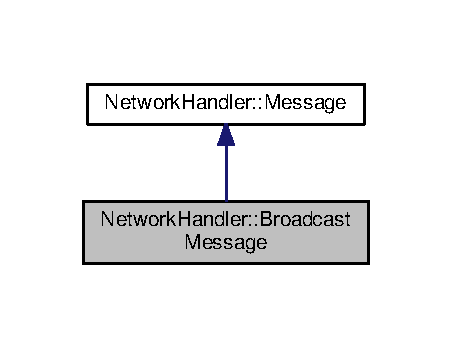
\includegraphics[width=217pt]{structNetworkHandler_1_1BroadcastMessage__inherit__graph}
\end{center}
\end{figure}


Collaboration diagram for Network\+Handler\+:\+:Broadcast\+Message\+:\nopagebreak
\begin{figure}[H]
\begin{center}
\leavevmode
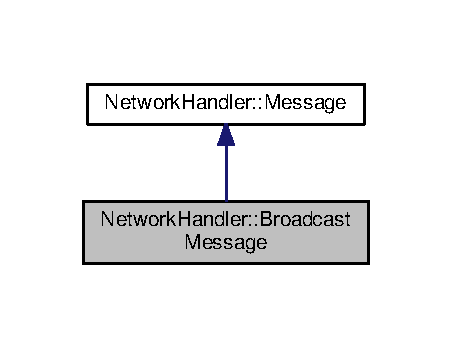
\includegraphics[width=217pt]{structNetworkHandler_1_1BroadcastMessage__coll__graph}
\end{center}
\end{figure}
\subsection*{Public Attributes}
\begin{DoxyCompactItemize}
\item 
\mbox{\Hypertarget{structNetworkHandler_1_1BroadcastMessage_ae41fb3a119ecb6dcc8e0bd7b30bba836}\label{structNetworkHandler_1_1BroadcastMessage_ae41fb3a119ecb6dcc8e0bd7b30bba836}} 
uint32\+\_\+t \mbox{\hyperlink{structNetworkHandler_1_1BroadcastMessage_ae41fb3a119ecb6dcc8e0bd7b30bba836}{rgb\+Ceiling}}
\begin{DoxyCompactList}\small\item\em R\+GB ceiling value of sender unit. \end{DoxyCompactList}\item 
\mbox{\Hypertarget{structNetworkHandler_1_1BroadcastMessage_a60dfde06603616556ccda32917408f4e}\label{structNetworkHandler_1_1BroadcastMessage_a60dfde06603616556ccda32917408f4e}} 
uint32\+\_\+t \mbox{\hyperlink{structNetworkHandler_1_1BroadcastMessage_a60dfde06603616556ccda32917408f4e}{rgb\+Wall}}
\begin{DoxyCompactList}\small\item\em R\+GB wall value of sender unit. \end{DoxyCompactList}\item 
\mbox{\Hypertarget{structNetworkHandler_1_1BroadcastMessage_a759ee3b4d1f21f4f5fd107f943f6b984}\label{structNetworkHandler_1_1BroadcastMessage_a759ee3b4d1f21f4f5fd107f943f6b984}} 
char \mbox{\hyperlink{structNetworkHandler_1_1BroadcastMessage_a759ee3b4d1f21f4f5fd107f943f6b984}{description}} \mbox{[}16\mbox{]}
\begin{DoxyCompactList}\small\item\em Description of sender unit. \end{DoxyCompactList}\item 
\mbox{\Hypertarget{structNetworkHandler_1_1BroadcastMessage_a7e3e051c6a20003c7ee62649a80b4dcd}\label{structNetworkHandler_1_1BroadcastMessage_a7e3e051c6a20003c7ee62649a80b4dcd}} 
uint16\+\_\+t \mbox{\hyperlink{structNetworkHandler_1_1BroadcastMessage_a7e3e051c6a20003c7ee62649a80b4dcd}{image}} \mbox{[}256\mbox{]}
\begin{DoxyCompactList}\small\item\em Icon of sender unitt. \end{DoxyCompactList}\end{DoxyCompactItemize}


\subsection{Detailed Description}
Broadcast message. Type 0. 

The documentation for this struct was generated from the following file\+:\begin{DoxyCompactItemize}
\item 
Network/Network\+Handler.\+h\end{DoxyCompactItemize}

\hypertarget{classScreen_1_1ColorSquareLineElement}{}\section{Screen\+:\+:Color\+Square\+Line\+Element Class Reference}
\label{classScreen_1_1ColorSquareLineElement}\index{Screen\+::\+Color\+Square\+Line\+Element@{Screen\+::\+Color\+Square\+Line\+Element}}


Inheritance diagram for Screen\+:\+:Color\+Square\+Line\+Element\+:

\hypertarget{structNetworkHandler_1_1ControlMessage}{}\section{Network\+Handler\+:\+:Control\+Message Struct Reference}
\label{structNetworkHandler_1_1ControlMessage}\index{Network\+Handler\+::\+Control\+Message@{Network\+Handler\+::\+Control\+Message}}


Control message. Types 1 and 2.  




{\ttfamily \#include $<$Network\+Handler.\+h$>$}



Inheritance diagram for Network\+Handler\+:\+:Control\+Message\+:\nopagebreak
\begin{figure}[H]
\begin{center}
\leavevmode
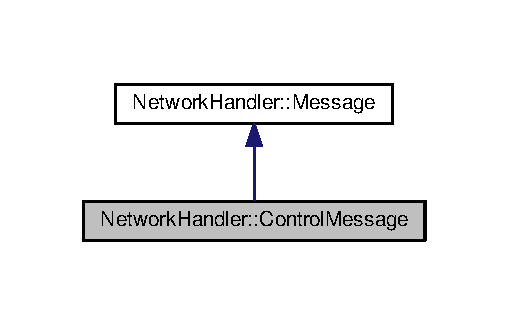
\includegraphics[width=244pt]{structNetworkHandler_1_1ControlMessage__inherit__graph}
\end{center}
\end{figure}


Collaboration diagram for Network\+Handler\+:\+:Control\+Message\+:\nopagebreak
\begin{figure}[H]
\begin{center}
\leavevmode
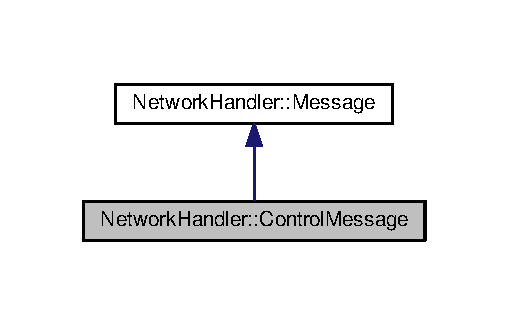
\includegraphics[width=244pt]{structNetworkHandler_1_1ControlMessage__coll__graph}
\end{center}
\end{figure}
\subsection*{Public Attributes}
\begin{DoxyCompactItemize}
\item 
\mbox{\Hypertarget{structNetworkHandler_1_1ControlMessage_ac24f313f593e8fe3406f9ae54201513a}\label{structNetworkHandler_1_1ControlMessage_ac24f313f593e8fe3406f9ae54201513a}} 
int16\+\_\+t \mbox{\hyperlink{structNetworkHandler_1_1ControlMessage_ac24f313f593e8fe3406f9ae54201513a}{values\+Ceiling}} \mbox{[}3\mbox{]}
\begin{DoxyCompactList}\small\item\em Ceiling values to increment/set for the recieving unit. \end{DoxyCompactList}\item 
\mbox{\Hypertarget{structNetworkHandler_1_1ControlMessage_a6d54372eb881b32e6face646afaaea86}\label{structNetworkHandler_1_1ControlMessage_a6d54372eb881b32e6face646afaaea86}} 
int16\+\_\+t \mbox{\hyperlink{structNetworkHandler_1_1ControlMessage_a6d54372eb881b32e6face646afaaea86}{values\+Wall}} \mbox{[}3\mbox{]}
\begin{DoxyCompactList}\small\item\em Wall values to increment/set for the recieving unit. \end{DoxyCompactList}\end{DoxyCompactItemize}


\subsection{Detailed Description}
Control message. Types 1 and 2. 

Type 1 increments values. Type 2 sets values. 

The documentation for this struct was generated from the following file\+:\begin{DoxyCompactItemize}
\item 
Network/Network\+Handler.\+h\end{DoxyCompactItemize}

\hypertarget{structControlMessageQueue_1_1ControlMessageInfo}{}\section{Control\+Message\+Queue\+:\+:Control\+Message\+Info Struct Reference}
\label{structControlMessageQueue_1_1ControlMessageInfo}\index{Control\+Message\+Queue\+::\+Control\+Message\+Info@{Control\+Message\+Queue\+::\+Control\+Message\+Info}}


Element of the \mbox{\hyperlink{classControlMessageQueue}{Control\+Message\+Queue}}.  




{\ttfamily \#include $<$Control\+Message\+Queue.\+h$>$}

\subsection*{Public Member Functions}
\begin{DoxyCompactItemize}
\item 
\mbox{\Hypertarget{structControlMessageQueue_1_1ControlMessageInfo_a2e85f6e0583ea739ff6ec35ef1655bef}\label{structControlMessageQueue_1_1ControlMessageInfo_a2e85f6e0583ea739ff6ec35ef1655bef}} 
\mbox{\hyperlink{structControlMessageQueue_1_1ControlMessageInfo_a2e85f6e0583ea739ff6ec35ef1655bef}{Control\+Message\+Info}} ()
\begin{DoxyCompactList}\small\item\em Empty constructor constructs invalid \mbox{\hyperlink{structControlMessageQueue_1_1ControlMessageInfo}{Control\+Message\+Info}}. \end{DoxyCompactList}\item 
\mbox{\hyperlink{structControlMessageQueue_1_1ControlMessageInfo_a86967ffe7674cc77dcb2ddae8917dc32}{Control\+Message\+Info}} (uint32\+\_\+t \mbox{\hyperlink{structControlMessageQueue_1_1ControlMessageInfo_a9c729d9dd8e2bbabfbdfcdaf845065f6}{ip}}, int \mbox{\hyperlink{structControlMessageQueue_1_1ControlMessageInfo_a0166019e4c749c1fcea08074c641af3e}{type}}=-\/1)
\begin{DoxyCompactList}\small\item\em \mbox{\hyperlink{structControlMessageQueue_1_1ControlMessageInfo}{Control\+Message\+Info}} constructor with ip and optional type. \end{DoxyCompactList}\end{DoxyCompactItemize}
\subsection*{Public Attributes}
\begin{DoxyCompactItemize}
\item 
\mbox{\Hypertarget{structControlMessageQueue_1_1ControlMessageInfo_a9c729d9dd8e2bbabfbdfcdaf845065f6}\label{structControlMessageQueue_1_1ControlMessageInfo_a9c729d9dd8e2bbabfbdfcdaf845065f6}} 
uint32\+\_\+t \mbox{\hyperlink{structControlMessageQueue_1_1ControlMessageInfo_a9c729d9dd8e2bbabfbdfcdaf845065f6}{ip}}
\begin{DoxyCompactList}\small\item\em IP address. \end{DoxyCompactList}\item 
\mbox{\Hypertarget{structControlMessageQueue_1_1ControlMessageInfo_a0166019e4c749c1fcea08074c641af3e}\label{structControlMessageQueue_1_1ControlMessageInfo_a0166019e4c749c1fcea08074c641af3e}} 
int \mbox{\hyperlink{structControlMessageQueue_1_1ControlMessageInfo_a0166019e4c749c1fcea08074c641af3e}{type}}
\begin{DoxyCompactList}\small\item\em Message type. \end{DoxyCompactList}\item 
\mbox{\Hypertarget{structControlMessageQueue_1_1ControlMessageInfo_aab343940b8582a6f6b0a36b16879b685}\label{structControlMessageQueue_1_1ControlMessageInfo_aab343940b8582a6f6b0a36b16879b685}} 
int16\+\_\+t \mbox{\hyperlink{structControlMessageQueue_1_1ControlMessageInfo_aab343940b8582a6f6b0a36b16879b685}{values\+Ceiling}} \mbox{[}3\mbox{]}
\begin{DoxyCompactList}\small\item\em Values ceiling. \end{DoxyCompactList}\item 
\mbox{\Hypertarget{structControlMessageQueue_1_1ControlMessageInfo_a7a3bd15c760863933774d32359cf4411}\label{structControlMessageQueue_1_1ControlMessageInfo_a7a3bd15c760863933774d32359cf4411}} 
int16\+\_\+t \mbox{\hyperlink{structControlMessageQueue_1_1ControlMessageInfo_a7a3bd15c760863933774d32359cf4411}{values\+Wall}} \mbox{[}3\mbox{]}
\begin{DoxyCompactList}\small\item\em Values wall. \end{DoxyCompactList}\end{DoxyCompactItemize}


\subsection{Detailed Description}
Element of the \mbox{\hyperlink{classControlMessageQueue}{Control\+Message\+Queue}}. 

\begin{DoxySeeAlso}{See also}
\mbox{\hyperlink{structNetworkHandler_1_1Message}{Network\+Handler\+::\+Message}} 

\mbox{\hyperlink{structNetworkHandler_1_1ControlMessage}{Network\+Handler\+::\+Control\+Message}} 
\end{DoxySeeAlso}


\subsection{Constructor \& Destructor Documentation}
\mbox{\Hypertarget{structControlMessageQueue_1_1ControlMessageInfo_a86967ffe7674cc77dcb2ddae8917dc32}\label{structControlMessageQueue_1_1ControlMessageInfo_a86967ffe7674cc77dcb2ddae8917dc32}} 
\index{Control\+Message\+Queue\+::\+Control\+Message\+Info@{Control\+Message\+Queue\+::\+Control\+Message\+Info}!Control\+Message\+Info@{Control\+Message\+Info}}
\index{Control\+Message\+Info@{Control\+Message\+Info}!Control\+Message\+Queue\+::\+Control\+Message\+Info@{Control\+Message\+Queue\+::\+Control\+Message\+Info}}
\subsubsection{\texorpdfstring{Control\+Message\+Info()}{ControlMessageInfo()}}
{\footnotesize\ttfamily Control\+Message\+Queue\+::\+Control\+Message\+Info\+::\+Control\+Message\+Info (\begin{DoxyParamCaption}\item[{uint32\+\_\+t}]{ip,  }\item[{int}]{type = {\ttfamily -\/1} }\end{DoxyParamCaption})\hspace{0.3cm}{\ttfamily [inline]}}



\mbox{\hyperlink{structControlMessageQueue_1_1ControlMessageInfo}{Control\+Message\+Info}} constructor with ip and optional type. 

If type is set to 2, this constructor also sets all values to -\/1. 
\begin{DoxyParams}[1]{Parameters}
\mbox{\tt in}  & {\em ip} & \\
\hline
\mbox{\tt in}  & {\em type} & \\
\hline
\end{DoxyParams}


The documentation for this struct was generated from the following file\+:\begin{DoxyCompactItemize}
\item 
Misc/Control\+Message\+Queue.\+h\end{DoxyCompactItemize}

\hypertarget{classControlMessageQueue}{}\section{Control\+Message\+Queue Class Reference}
\label{classControlMessageQueue}\index{Control\+Message\+Queue@{Control\+Message\+Queue}}


Thread-\/safe F\+I\+FO queue for control messages.  




{\ttfamily \#include $<$Control\+Message\+Queue.\+h$>$}

\subsection*{Classes}
\begin{DoxyCompactItemize}
\item 
struct \mbox{\hyperlink{structControlMessageQueue_1_1ControlMessageInfo}{Control\+Message\+Info}}
\begin{DoxyCompactList}\small\item\em Element of the \mbox{\hyperlink{classControlMessageQueue}{Control\+Message\+Queue}}. \end{DoxyCompactList}\end{DoxyCompactItemize}
\subsection*{Public Types}
\begin{DoxyCompactItemize}
\item 
typedef struct \mbox{\hyperlink{structControlMessageQueue_1_1ControlMessageInfo}{Control\+Message\+Queue\+::\+Control\+Message\+Info}} \mbox{\hyperlink{classControlMessageQueue_a50df92d449dae01e49fd0e836c7d1f2e}{Control\+Message\+Info}}
\begin{DoxyCompactList}\small\item\em Element of the \mbox{\hyperlink{classControlMessageQueue}{Control\+Message\+Queue}}. \end{DoxyCompactList}\end{DoxyCompactItemize}
\subsection*{Public Member Functions}
\begin{DoxyCompactItemize}
\item 
bool \mbox{\hyperlink{classControlMessageQueue_ad0d97de85cb34b781fde757b665fb22e}{has\+Changed}} ()
\begin{DoxyCompactList}\small\item\em Checks if the queue has changed. \end{DoxyCompactList}\item 
size\+\_\+t \mbox{\hyperlink{classControlMessageQueue_a3b2d120facfc58fcdc315a806d76851a}{size}} ()
\begin{DoxyCompactList}\small\item\em Returns number of elements in the queue. \end{DoxyCompactList}\item 
void \mbox{\hyperlink{classControlMessageQueue_a766bed9ca18a663bba82cc32c253049a}{enqueue}} (\mbox{\hyperlink{structControlMessageQueue_1_1ControlMessageInfo}{Control\+Message\+Info}} info)
\begin{DoxyCompactList}\small\item\em Equeues an element at the back. \end{DoxyCompactList}\item 
\mbox{\hyperlink{structControlMessageQueue_1_1ControlMessageInfo}{Control\+Message\+Info}} \mbox{\hyperlink{classControlMessageQueue_a95142f7602e0a64b38a8f1cb02ef9497}{dequeue}} ()
\begin{DoxyCompactList}\small\item\em Dequeues an element from the front. \end{DoxyCompactList}\end{DoxyCompactItemize}


\subsection{Detailed Description}
Thread-\/safe F\+I\+FO queue for control messages. 

\subsection{Member Typedef Documentation}
\mbox{\Hypertarget{classControlMessageQueue_a50df92d449dae01e49fd0e836c7d1f2e}\label{classControlMessageQueue_a50df92d449dae01e49fd0e836c7d1f2e}} 
\index{Control\+Message\+Queue@{Control\+Message\+Queue}!Control\+Message\+Info@{Control\+Message\+Info}}
\index{Control\+Message\+Info@{Control\+Message\+Info}!Control\+Message\+Queue@{Control\+Message\+Queue}}
\subsubsection{\texorpdfstring{Control\+Message\+Info}{ControlMessageInfo}}
{\footnotesize\ttfamily typedef struct \mbox{\hyperlink{structControlMessageQueue_1_1ControlMessageInfo}{Control\+Message\+Queue\+::\+Control\+Message\+Info}}  \mbox{\hyperlink{structControlMessageQueue_1_1ControlMessageInfo}{Control\+Message\+Queue\+::\+Control\+Message\+Info}}}



Element of the \mbox{\hyperlink{classControlMessageQueue}{Control\+Message\+Queue}}. 

\begin{DoxySeeAlso}{See also}
\mbox{\hyperlink{structNetworkHandler_1_1Message}{Network\+Handler\+::\+Message}} 

\mbox{\hyperlink{structNetworkHandler_1_1ControlMessage}{Network\+Handler\+::\+Control\+Message}} 
\end{DoxySeeAlso}


\subsection{Member Function Documentation}
\mbox{\Hypertarget{classControlMessageQueue_a95142f7602e0a64b38a8f1cb02ef9497}\label{classControlMessageQueue_a95142f7602e0a64b38a8f1cb02ef9497}} 
\index{Control\+Message\+Queue@{Control\+Message\+Queue}!dequeue@{dequeue}}
\index{dequeue@{dequeue}!Control\+Message\+Queue@{Control\+Message\+Queue}}
\subsubsection{\texorpdfstring{dequeue()}{dequeue()}}
{\footnotesize\ttfamily \mbox{\hyperlink{structControlMessageQueue_1_1ControlMessageInfo}{Control\+Message\+Queue\+::\+Control\+Message\+Info}} Control\+Message\+Queue\+::dequeue (\begin{DoxyParamCaption}{ }\end{DoxyParamCaption})}



Dequeues an element from the front. 

\begin{DoxyReturn}{Returns}
The front element. If there are no elements, returns \mbox{\hyperlink{classControlMessageQueue_a50df92d449dae01e49fd0e836c7d1f2e}{Control\+Message\+Info()}}; 
\end{DoxyReturn}
\mbox{\Hypertarget{classControlMessageQueue_a766bed9ca18a663bba82cc32c253049a}\label{classControlMessageQueue_a766bed9ca18a663bba82cc32c253049a}} 
\index{Control\+Message\+Queue@{Control\+Message\+Queue}!enqueue@{enqueue}}
\index{enqueue@{enqueue}!Control\+Message\+Queue@{Control\+Message\+Queue}}
\subsubsection{\texorpdfstring{enqueue()}{enqueue()}}
{\footnotesize\ttfamily void Control\+Message\+Queue\+::enqueue (\begin{DoxyParamCaption}\item[{\mbox{\hyperlink{structControlMessageQueue_1_1ControlMessageInfo}{Control\+Message\+Queue\+::\+Control\+Message\+Info}}}]{info }\end{DoxyParamCaption})}



Equeues an element at the back. 


\begin{DoxyParams}[1]{Parameters}
\mbox{\tt in}  & {\em info} & \\
\hline
\end{DoxyParams}
\mbox{\Hypertarget{classControlMessageQueue_ad0d97de85cb34b781fde757b665fb22e}\label{classControlMessageQueue_ad0d97de85cb34b781fde757b665fb22e}} 
\index{Control\+Message\+Queue@{Control\+Message\+Queue}!has\+Changed@{has\+Changed}}
\index{has\+Changed@{has\+Changed}!Control\+Message\+Queue@{Control\+Message\+Queue}}
\subsubsection{\texorpdfstring{has\+Changed()}{hasChanged()}}
{\footnotesize\ttfamily bool Control\+Message\+Queue\+::has\+Changed (\begin{DoxyParamCaption}{ }\end{DoxyParamCaption})}



Checks if the queue has changed. 

\begin{DoxyReturn}{Returns}
Value indicating whether the queue has changed since the last call to this function. 
\end{DoxyReturn}
\mbox{\Hypertarget{classControlMessageQueue_a3b2d120facfc58fcdc315a806d76851a}\label{classControlMessageQueue_a3b2d120facfc58fcdc315a806d76851a}} 
\index{Control\+Message\+Queue@{Control\+Message\+Queue}!size@{size}}
\index{size@{size}!Control\+Message\+Queue@{Control\+Message\+Queue}}
\subsubsection{\texorpdfstring{size()}{size()}}
{\footnotesize\ttfamily size\+\_\+t Control\+Message\+Queue\+::size (\begin{DoxyParamCaption}{ }\end{DoxyParamCaption})}



Returns number of elements in the queue. 

\begin{DoxyReturn}{Returns}
Number of elements in the queue. 
\end{DoxyReturn}


The documentation for this class was generated from the following files\+:\begin{DoxyCompactItemize}
\item 
Misc/Control\+Message\+Queue.\+h\item 
Misc/Control\+Message\+Queue.\+cpp\end{DoxyCompactItemize}

\hypertarget{classDeviceInput}{}\section{Device\+Input Class Reference}
\label{classDeviceInput}\index{Device\+Input@{Device\+Input}}
\subsection*{Public Member Functions}
\begin{DoxyCompactItemize}
\item 
\mbox{\hyperlink{classDeviceInput_a5a5d144c0a4a2d0fedfd85fcb687a716}{Device\+Input}} ()
\item 
\mbox{\hyperlink{classDeviceInput_a6c06d020cca58b3d4763e1717382b1a8}{$\sim$\+Device\+Input}} ()
\item 
\mbox{\Hypertarget{classDeviceInput_ae6af261f4e6fa656dad4bd4a1efddbc6}\label{classDeviceInput_ae6af261f4e6fa656dad4bd4a1efddbc6}} 
void \mbox{\hyperlink{classDeviceInput_ae6af261f4e6fa656dad4bd4a1efddbc6}{update}} ()
\begin{DoxyCompactList}\small\item\em Gets the input (knobs state) from the device. \end{DoxyCompactList}\end{DoxyCompactItemize}
\subsection*{Public Attributes}
\begin{DoxyCompactItemize}
\item 
\mbox{\Hypertarget{classDeviceInput_a2dae4108527f110262644b6a2609a213}\label{classDeviceInput_a2dae4108527f110262644b6a2609a213}} 
int8\+\_\+t \mbox{\hyperlink{classDeviceInput_a2dae4108527f110262644b6a2609a213}{R\+G\+B\+Delta}} \mbox{[}3\mbox{]}
\begin{DoxyCompactList}\small\item\em The change in the device knob positions. \end{DoxyCompactList}\item 
\mbox{\Hypertarget{classDeviceInput_a27dd22c6d022b77c645899a8793d511a}\label{classDeviceInput_a27dd22c6d022b77c645899a8793d511a}} 
bool \mbox{\hyperlink{classDeviceInput_a27dd22c6d022b77c645899a8793d511a}{R\+G\+B\+Pressed}} \mbox{[}3\mbox{]}
\begin{DoxyCompactList}\small\item\em Wether given device knob is pressed or not. \end{DoxyCompactList}\end{DoxyCompactItemize}


\subsection{Constructor \& Destructor Documentation}
\mbox{\Hypertarget{classDeviceInput_a5a5d144c0a4a2d0fedfd85fcb687a716}\label{classDeviceInput_a5a5d144c0a4a2d0fedfd85fcb687a716}} 
\index{Device\+Input@{Device\+Input}!Device\+Input@{Device\+Input}}
\index{Device\+Input@{Device\+Input}!Device\+Input@{Device\+Input}}
\subsubsection{\texorpdfstring{Device\+Input()}{DeviceInput()}}
{\footnotesize\ttfamily Device\+Input\+::\+Device\+Input (\begin{DoxyParamCaption}{ }\end{DoxyParamCaption})}

Constructor. \mbox{\Hypertarget{classDeviceInput_a6c06d020cca58b3d4763e1717382b1a8}\label{classDeviceInput_a6c06d020cca58b3d4763e1717382b1a8}} 
\index{Device\+Input@{Device\+Input}!````~Device\+Input@{$\sim$\+Device\+Input}}
\index{````~Device\+Input@{$\sim$\+Device\+Input}!Device\+Input@{Device\+Input}}
\subsubsection{\texorpdfstring{$\sim$\+Device\+Input()}{~DeviceInput()}}
{\footnotesize\ttfamily Device\+Input\+::$\sim$\+Device\+Input (\begin{DoxyParamCaption}{ }\end{DoxyParamCaption})}

Destructor. 

The documentation for this class was generated from the following files\+:\begin{DoxyCompactItemize}
\item 
M\+Z\+Api/Device\+Input.\+h\item 
M\+Z\+Api/Device\+Input.\+cpp\end{DoxyCompactItemize}

\hypertarget{classDisplay}{}\section{Display Class Reference}
\label{classDisplay}\index{Display@{Display}}
\subsection*{Public Member Functions}
\begin{DoxyCompactItemize}
\item 
\hyperlink{classDisplay_a579fdca9754b50088f77dcb7ba3489ac}{Display} (uint16\+\_\+t bg\+Colour, uint16\+\_\+t fg\+Colour, uint16\+\_\+t highlight\+Colour, \hyperlink{structfont__descriptor__t}{font\+\_\+descriptor\+\_\+t} font)
\begin{DoxyCompactList}\small\item\em The display constructor taking colours and fonts as parameters. \end{DoxyCompactList}\item 
\hyperlink{classDisplay_ac2607a6bb236c55547a4223d40d85d1f}{$\sim$\+Display} ()\hypertarget{classDisplay_ac2607a6bb236c55547a4223d40d85d1f}{}\label{classDisplay_ac2607a6bb236c55547a4223d40d85d1f}

\begin{DoxyCompactList}\small\item\em The display destructor. \end{DoxyCompactList}\item 
void \hyperlink{classDisplay_aa68ef5d785a1a96abdfe0a0f8ccdc379}{handle\+Input} (int8\+\_\+t rgb\+Delta\mbox{[}3\mbox{]}, bool knobs\+Pressed\mbox{[}3\mbox{]})
\begin{DoxyCompactList}\small\item\em Reacts to input from the device. \end{DoxyCompactList}\item 
void \hyperlink{classDisplay_a566e7cbce9f606a20787c6d42c189dc2}{switch\+Screen} (\hyperlink{classScreen}{Screen} $\ast$new\+Screen)
\begin{DoxyCompactList}\small\item\em Changes the display screen. \end{DoxyCompactList}\item 
bool \hyperlink{classDisplay_ad043404964c19f51bb903da796aaefda}{to\+Previous\+Screen} (bool keep\+Alive=false)
\begin{DoxyCompactList}\small\item\em Returns to the previous screen. \end{DoxyCompactList}\item 
void \hyperlink{classDisplay_a8292ad87dddbf7090e074bcff5968d93}{set\+Colours} (uint16\+\_\+t bg\+Colour, uint16\+\_\+t fg\+Colour, uint16\+\_\+t highlight\+Colour)
\begin{DoxyCompactList}\small\item\em Sets the base colours for the display -\/ background, foreground and highlight. \end{DoxyCompactList}\item 
void \hyperlink{classDisplay_afb2154f5edc1c2784ef43d0ddae9cd6d}{set\+Font} (\hyperlink{structfont__descriptor__t}{font\+\_\+descriptor\+\_\+t} font)
\begin{DoxyCompactList}\small\item\em Sets the font for the display. \end{DoxyCompactList}\item 
void {\bfseries test\+Display} ()\hypertarget{classDisplay_a98fd128bf53a5831c18a3e2af6309cca}{}\label{classDisplay_a98fd128bf53a5831c18a3e2af6309cca}

\item 
void \hyperlink{classDisplay_a905f9f783556b52da4655c541a5e3ea0}{clear\+Screen} (uint16\+\_\+t colour)
\begin{DoxyCompactList}\small\item\em Sets the whole display to one colour. \end{DoxyCompactList}\item 
void \hyperlink{classDisplay_a34d1063149dc9f36c43afd5066b0b3ce}{set\+Pixel} (int x, int y, uint16\+\_\+t colour)
\begin{DoxyCompactList}\small\item\em Sets one pixel to a given colour. \end{DoxyCompactList}\item 
void \hyperlink{classDisplay_aeadae3356ab6ef6bc101dd5c3ee1317d}{render\+Rectangle} (int left, int top, int right, int bottom, uint16\+\_\+t colour)
\begin{DoxyCompactList}\small\item\em Renders an axis-\/aligned rectangle with given corner points in a given colour. \end{DoxyCompactList}\item 
void \hyperlink{classDisplay_a94ad8f357b5fffdd4711a593e29003a8}{render\+Colour\+Square} (int topX, int topY, uint16\+\_\+t colour)
\begin{DoxyCompactList}\small\item\em Renders an axis-\/aligned rectangle with given position in a given colour. \end{DoxyCompactList}\item 
void \hyperlink{classDisplay_a9e72ead0a3cb23753b1fba042926ce88}{render\+Text} (int topX, int topY, std\+::string text, uint16\+\_\+t colour)
\begin{DoxyCompactList}\small\item\em Renders an axis-\/aligned text-\/line starting at a given position in a given colour. \end{DoxyCompactList}\item 
void \hyperlink{classDisplay_ad50ca28eb1147af9d31316bd2ad8ef6e}{render\+Icon} (uint16\+\_\+t $\ast$buffer, int topX, int topY)
\begin{DoxyCompactList}\small\item\em Renders an icon starting at a given position. \end{DoxyCompactList}\item 
void \hyperlink{classDisplay_a4fe6059ab67f9a11469ea53f4a5ddb0d}{redraw} ()\hypertarget{classDisplay_a4fe6059ab67f9a11469ea53f4a5ddb0d}{}\label{classDisplay_a4fe6059ab67f9a11469ea53f4a5ddb0d}

\begin{DoxyCompactList}\small\item\em Renders the display buffer on the device. \end{DoxyCompactList}\end{DoxyCompactItemize}
\subsection*{Public Attributes}
\begin{DoxyCompactItemize}
\item 
uint16\+\_\+t {\bfseries fg\+Colour}\hypertarget{classDisplay_aa6a2bd6e8f05a0794ff6b32c30723245}{}\label{classDisplay_aa6a2bd6e8f05a0794ff6b32c30723245}

\item 
uint16\+\_\+t {\bfseries bg\+Colour}\hypertarget{classDisplay_a23a0f9867d7ba82c45a3c612c84e0504}{}\label{classDisplay_a23a0f9867d7ba82c45a3c612c84e0504}

\item 
uint16\+\_\+t \hyperlink{classDisplay_a1487285b39c53295e92cad6b3074a924}{select\+Colour}
\item 
size\+\_\+t \hyperlink{classDisplay_a7183e09a442a157a00391639a34cd4d8}{line\+Max}
\end{DoxyCompactItemize}
\subsection*{Static Public Attributes}
\begin{DoxyCompactItemize}
\item 
static const size\+\_\+t \hyperlink{classDisplay_a6f1dec624224569510e05c937d33ac4d}{width} = 480
\item 
static const size\+\_\+t \hyperlink{classDisplay_ac677f0db63e8eef2373fe84791cad17c}{height} = 320
\end{DoxyCompactItemize}


\subsection{Constructor \& Destructor Documentation}
\index{Display@{Display}!Display@{Display}}
\index{Display@{Display}!Display@{Display}}
\subsubsection[{\texorpdfstring{Display(uint16\+\_\+t bg\+Colour, uint16\+\_\+t fg\+Colour, uint16\+\_\+t highlight\+Colour, font\+\_\+descriptor\+\_\+t font)}{Display(uint16_t bgColour, uint16_t fgColour, uint16_t highlightColour, font_descriptor_t font)}}]{\setlength{\rightskip}{0pt plus 5cm}Display\+::\+Display (
\begin{DoxyParamCaption}
\item[{uint16\+\_\+t}]{bg\+Colour, }
\item[{uint16\+\_\+t}]{fg\+Colour, }
\item[{uint16\+\_\+t}]{highlight\+Colour, }
\item[{{\bf font\+\_\+descriptor\+\_\+t}}]{font}
\end{DoxyParamCaption}
)}\hypertarget{classDisplay_a579fdca9754b50088f77dcb7ba3489ac}{}\label{classDisplay_a579fdca9754b50088f77dcb7ba3489ac}


The display constructor taking colours and fonts as parameters. 


\begin{DoxyParams}{Parameters}
{\em bg\+Colour} & The colour used for background. \\
\hline
{\em fg\+Colour} & The colour used for foreground. \\
\hline
{\em highlight\+Colour} & The colour used for highlighted items, such as the sleected ones. \\
\hline
{\em font} & The font to be used for displayed text. \\
\hline
\end{DoxyParams}


\subsection{Member Function Documentation}
\index{Display@{Display}!clear\+Screen@{clear\+Screen}}
\index{clear\+Screen@{clear\+Screen}!Display@{Display}}
\subsubsection[{\texorpdfstring{clear\+Screen(uint16\+\_\+t colour)}{clearScreen(uint16_t colour)}}]{\setlength{\rightskip}{0pt plus 5cm}void Display\+::clear\+Screen (
\begin{DoxyParamCaption}
\item[{uint16\+\_\+t}]{colour}
\end{DoxyParamCaption}
)}\hypertarget{classDisplay_a905f9f783556b52da4655c541a5e3ea0}{}\label{classDisplay_a905f9f783556b52da4655c541a5e3ea0}


Sets the whole display to one colour. 


\begin{DoxyParams}{Parameters}
{\em colour} & The colour used as background. \\
\hline
\end{DoxyParams}
\index{Display@{Display}!handle\+Input@{handle\+Input}}
\index{handle\+Input@{handle\+Input}!Display@{Display}}
\subsubsection[{\texorpdfstring{handle\+Input(int8\+\_\+t rgb\+Delta[3], bool knobs\+Pressed[3])}{handleInput(int8_t rgbDelta[3], bool knobsPressed[3])}}]{\setlength{\rightskip}{0pt plus 5cm}void Display\+::handle\+Input (
\begin{DoxyParamCaption}
\item[{int8\+\_\+t}]{rgb\+Delta\mbox{[}3\mbox{]}, }
\item[{bool}]{knobs\+Pressed\mbox{[}3\mbox{]}}
\end{DoxyParamCaption}
)}\hypertarget{classDisplay_aa68ef5d785a1a96abdfe0a0f8ccdc379}{}\label{classDisplay_aa68ef5d785a1a96abdfe0a0f8ccdc379}


Reacts to input from the device. 


\begin{DoxyParams}{Parameters}
{\em rgb\+Delta} & The change in knobs position. \\
\hline
{\em knobs\+Pressed} & The high/low state of the knobs. \\
\hline
\end{DoxyParams}
\index{Display@{Display}!render\+Colour\+Square@{render\+Colour\+Square}}
\index{render\+Colour\+Square@{render\+Colour\+Square}!Display@{Display}}
\subsubsection[{\texorpdfstring{render\+Colour\+Square(int top\+X, int top\+Y, uint16\+\_\+t colour)}{renderColourSquare(int topX, int topY, uint16_t colour)}}]{\setlength{\rightskip}{0pt plus 5cm}void Display\+::render\+Colour\+Square (
\begin{DoxyParamCaption}
\item[{int}]{topX, }
\item[{int}]{topY, }
\item[{uint16\+\_\+t}]{colour}
\end{DoxyParamCaption}
)}\hypertarget{classDisplay_a94ad8f357b5fffdd4711a593e29003a8}{}\label{classDisplay_a94ad8f357b5fffdd4711a593e29003a8}


Renders an axis-\/aligned rectangle with given position in a given colour. 


\begin{DoxyParams}{Parameters}
{\em left} & The x coordinate of the left edge. \\
\hline
{\em top} & The y coordinate of the top edge. \\
\hline
{\em right} & The x cooridnate of the right edge. \\
\hline
{\em bottom} & The y coordinate of the bottom edgge. \\
\hline
{\em colour} & The colour of the rectangle. \\
\hline
\end{DoxyParams}
\index{Display@{Display}!render\+Icon@{render\+Icon}}
\index{render\+Icon@{render\+Icon}!Display@{Display}}
\subsubsection[{\texorpdfstring{render\+Icon(uint16\+\_\+t $\ast$buffer, int top\+X, int top\+Y)}{renderIcon(uint16_t *buffer, int topX, int topY)}}]{\setlength{\rightskip}{0pt plus 5cm}void Display\+::render\+Icon (
\begin{DoxyParamCaption}
\item[{uint16\+\_\+t $\ast$}]{buffer, }
\item[{int}]{topX, }
\item[{int}]{topY}
\end{DoxyParamCaption}
)}\hypertarget{classDisplay_ad50ca28eb1147af9d31316bd2ad8ef6e}{}\label{classDisplay_ad50ca28eb1147af9d31316bd2ad8ef6e}


Renders an icon starting at a given position. 


\begin{DoxyParams}{Parameters}
{\em buffer} & The 16x16 image to be rendered. \\
\hline
{\em topX} & The x coordinate of the top-\/left corner. \\
\hline
{\em topY} & The y coordinate of the top-\/left corner. \\
\hline
\end{DoxyParams}
\index{Display@{Display}!render\+Rectangle@{render\+Rectangle}}
\index{render\+Rectangle@{render\+Rectangle}!Display@{Display}}
\subsubsection[{\texorpdfstring{render\+Rectangle(int left, int top, int right, int bottom, uint16\+\_\+t colour)}{renderRectangle(int left, int top, int right, int bottom, uint16_t colour)}}]{\setlength{\rightskip}{0pt plus 5cm}void Display\+::render\+Rectangle (
\begin{DoxyParamCaption}
\item[{int}]{left, }
\item[{int}]{top, }
\item[{int}]{right, }
\item[{int}]{bottom, }
\item[{uint16\+\_\+t}]{colour}
\end{DoxyParamCaption}
)}\hypertarget{classDisplay_aeadae3356ab6ef6bc101dd5c3ee1317d}{}\label{classDisplay_aeadae3356ab6ef6bc101dd5c3ee1317d}


Renders an axis-\/aligned rectangle with given corner points in a given colour. 


\begin{DoxyParams}{Parameters}
{\em left} & The x coordinate of the left edge. \\
\hline
{\em top} & The y coordinate of the top edge. \\
\hline
{\em right} & The x cooridnate of the right edge. \\
\hline
{\em bottom} & The y coordinate of the bottom edgge. \\
\hline
{\em colour} & The colour of the rectangle. \\
\hline
\end{DoxyParams}
\index{Display@{Display}!render\+Text@{render\+Text}}
\index{render\+Text@{render\+Text}!Display@{Display}}
\subsubsection[{\texorpdfstring{render\+Text(int top\+X, int top\+Y, std\+::string text, uint16\+\_\+t colour)}{renderText(int topX, int topY, std::string text, uint16_t colour)}}]{\setlength{\rightskip}{0pt plus 5cm}void Display\+::render\+Text (
\begin{DoxyParamCaption}
\item[{int}]{topX, }
\item[{int}]{topY, }
\item[{std\+::string}]{text, }
\item[{uint16\+\_\+t}]{colour}
\end{DoxyParamCaption}
)}\hypertarget{classDisplay_a9e72ead0a3cb23753b1fba042926ce88}{}\label{classDisplay_a9e72ead0a3cb23753b1fba042926ce88}


Renders an axis-\/aligned text-\/line starting at a given position in a given colour. 


\begin{DoxyParams}{Parameters}
{\em topX} & The x coordinate of the top-\/left corner. \\
\hline
{\em topY} & The y coordinate of the top-\/left corner. \\
\hline
{\em text} & The text to be rendered. \\
\hline
{\em colour} & The colour of the text. \\
\hline
\end{DoxyParams}
\index{Display@{Display}!set\+Colours@{set\+Colours}}
\index{set\+Colours@{set\+Colours}!Display@{Display}}
\subsubsection[{\texorpdfstring{set\+Colours(uint16\+\_\+t bg\+Colour, uint16\+\_\+t fg\+Colour, uint16\+\_\+t highlight\+Colour)}{setColours(uint16_t bgColour, uint16_t fgColour, uint16_t highlightColour)}}]{\setlength{\rightskip}{0pt plus 5cm}void Display\+::set\+Colours (
\begin{DoxyParamCaption}
\item[{uint16\+\_\+t}]{bg\+Colour, }
\item[{uint16\+\_\+t}]{fg\+Colour, }
\item[{uint16\+\_\+t}]{highlight\+Colour}
\end{DoxyParamCaption}
)}\hypertarget{classDisplay_a8292ad87dddbf7090e074bcff5968d93}{}\label{classDisplay_a8292ad87dddbf7090e074bcff5968d93}


Sets the base colours for the display -\/ background, foreground and highlight. 


\begin{DoxyParams}{Parameters}
{\em bg\+Colour} & The colour used for background. \\
\hline
{\em fg\+Colour} & The colour used for foreground. \\
\hline
{\em highlight\+Colour} & The colour used for highlighted items, such as the sleected ones. \\
\hline
\end{DoxyParams}
\index{Display@{Display}!set\+Font@{set\+Font}}
\index{set\+Font@{set\+Font}!Display@{Display}}
\subsubsection[{\texorpdfstring{set\+Font(font\+\_\+descriptor\+\_\+t font)}{setFont(font_descriptor_t font)}}]{\setlength{\rightskip}{0pt plus 5cm}void Display\+::set\+Font (
\begin{DoxyParamCaption}
\item[{{\bf font\+\_\+descriptor\+\_\+t}}]{font}
\end{DoxyParamCaption}
)}\hypertarget{classDisplay_afb2154f5edc1c2784ef43d0ddae9cd6d}{}\label{classDisplay_afb2154f5edc1c2784ef43d0ddae9cd6d}


Sets the font for the display. 


\begin{DoxyParams}{Parameters}
{\em font} & The font to be used for displayed text. \\
\hline
\end{DoxyParams}
\index{Display@{Display}!set\+Pixel@{set\+Pixel}}
\index{set\+Pixel@{set\+Pixel}!Display@{Display}}
\subsubsection[{\texorpdfstring{set\+Pixel(int x, int y, uint16\+\_\+t colour)}{setPixel(int x, int y, uint16_t colour)}}]{\setlength{\rightskip}{0pt plus 5cm}void Display\+::set\+Pixel (
\begin{DoxyParamCaption}
\item[{int}]{x, }
\item[{int}]{y, }
\item[{uint16\+\_\+t}]{colour}
\end{DoxyParamCaption}
)}\hypertarget{classDisplay_a34d1063149dc9f36c43afd5066b0b3ce}{}\label{classDisplay_a34d1063149dc9f36c43afd5066b0b3ce}


Sets one pixel to a given colour. 


\begin{DoxyParams}{Parameters}
{\em x} & The pixel x coordinate. \\
\hline
{\em y} & The pixel y coordinate. \\
\hline
{\em colour} & The colour of the pixel. \\
\hline
\end{DoxyParams}
\index{Display@{Display}!switch\+Screen@{switch\+Screen}}
\index{switch\+Screen@{switch\+Screen}!Display@{Display}}
\subsubsection[{\texorpdfstring{switch\+Screen(\+Screen $\ast$new\+Screen)}{switchScreen(Screen *newScreen)}}]{\setlength{\rightskip}{0pt plus 5cm}void Display\+::switch\+Screen (
\begin{DoxyParamCaption}
\item[{{\bf Screen} $\ast$}]{new\+Screen}
\end{DoxyParamCaption}
)}\hypertarget{classDisplay_a566e7cbce9f606a20787c6d42c189dc2}{}\label{classDisplay_a566e7cbce9f606a20787c6d42c189dc2}


Changes the display screen. 


\begin{DoxyParams}{Parameters}
{\em new\+Screen} & The new screen. \\
\hline
\end{DoxyParams}
\index{Display@{Display}!to\+Previous\+Screen@{to\+Previous\+Screen}}
\index{to\+Previous\+Screen@{to\+Previous\+Screen}!Display@{Display}}
\subsubsection[{\texorpdfstring{to\+Previous\+Screen(bool keep\+Alive=false)}{toPreviousScreen(bool keepAlive=false)}}]{\setlength{\rightskip}{0pt plus 5cm}bool Display\+::to\+Previous\+Screen (
\begin{DoxyParamCaption}
\item[{bool}]{keep\+Alive = {\ttfamily false}}
\end{DoxyParamCaption}
)}\hypertarget{classDisplay_ad043404964c19f51bb903da796aaefda}{}\label{classDisplay_ad043404964c19f51bb903da796aaefda}


Returns to the previous screen. 


\begin{DoxyParams}{Parameters}
{\em keep\+Alive} & Whether the current screen should be preserved so that it can be returned to later. \\
\hline
\end{DoxyParams}
\begin{DoxyReturn}{Returns}

\end{DoxyReturn}


\subsection{Member Data Documentation}
\index{Display@{Display}!height@{height}}
\index{height@{height}!Display@{Display}}
\subsubsection[{\texorpdfstring{height}{height}}]{\setlength{\rightskip}{0pt plus 5cm}const size\+\_\+t Display\+::height = 320\hspace{0.3cm}{\ttfamily [static]}}\hypertarget{classDisplay_ac677f0db63e8eef2373fe84791cad17c}{}\label{classDisplay_ac677f0db63e8eef2373fe84791cad17c}
\hyperlink{classDisplay}{Display} height. \index{Display@{Display}!line\+Max@{line\+Max}}
\index{line\+Max@{line\+Max}!Display@{Display}}
\subsubsection[{\texorpdfstring{line\+Max}{lineMax}}]{\setlength{\rightskip}{0pt plus 5cm}size\+\_\+t Display\+::line\+Max}\hypertarget{classDisplay_a7183e09a442a157a00391639a34cd4d8}{}\label{classDisplay_a7183e09a442a157a00391639a34cd4d8}
The maximum number of lines that fit on the display. \index{Display@{Display}!select\+Colour@{select\+Colour}}
\index{select\+Colour@{select\+Colour}!Display@{Display}}
\subsubsection[{\texorpdfstring{select\+Colour}{selectColour}}]{\setlength{\rightskip}{0pt plus 5cm}uint16\+\_\+t Display\+::select\+Colour}\hypertarget{classDisplay_a1487285b39c53295e92cad6b3074a924}{}\label{classDisplay_a1487285b39c53295e92cad6b3074a924}
\hyperlink{classDisplay}{Display} colours. \index{Display@{Display}!width@{width}}
\index{width@{width}!Display@{Display}}
\subsubsection[{\texorpdfstring{width}{width}}]{\setlength{\rightskip}{0pt plus 5cm}const size\+\_\+t Display\+::width = 480\hspace{0.3cm}{\ttfamily [static]}}\hypertarget{classDisplay_a6f1dec624224569510e05c937d33ac4d}{}\label{classDisplay_a6f1dec624224569510e05c937d33ac4d}
\hyperlink{classDisplay}{Display} width. 

The documentation for this class was generated from the following files\+:\begin{DoxyCompactItemize}
\item 
M\+Z\+Api/Display.\+h\item 
M\+Z\+Api/Display.\+cpp\end{DoxyCompactItemize}

\hypertarget{structfont__descriptor__t}{}\section{font\+\_\+descriptor\+\_\+t Struct Reference}
\label{structfont__descriptor__t}\index{font\+\_\+descriptor\+\_\+t@{font\+\_\+descriptor\+\_\+t}}
\subsection*{Public Attributes}
\begin{DoxyCompactItemize}
\item 
char $\ast$ {\bfseries name}\hypertarget{structfont__descriptor__t_a7a5f7569c87f8995fe45b207897a0327}{}\label{structfont__descriptor__t_a7a5f7569c87f8995fe45b207897a0327}

\item 
int {\bfseries maxwidth}\hypertarget{structfont__descriptor__t_a8e21a73982523c96f1ca5f39487956a7}{}\label{structfont__descriptor__t_a8e21a73982523c96f1ca5f39487956a7}

\item 
unsigned int {\bfseries height}\hypertarget{structfont__descriptor__t_abf7d9548e4312aa8ab0b6c868c5c4ae3}{}\label{structfont__descriptor__t_abf7d9548e4312aa8ab0b6c868c5c4ae3}

\item 
int {\bfseries ascent}\hypertarget{structfont__descriptor__t_af23bcc2d3e1633f8153cb92df31de704}{}\label{structfont__descriptor__t_af23bcc2d3e1633f8153cb92df31de704}

\item 
int {\bfseries firstchar}\hypertarget{structfont__descriptor__t_a9d7d7a8a663625f6fb6120cb9dc0d970}{}\label{structfont__descriptor__t_a9d7d7a8a663625f6fb6120cb9dc0d970}

\item 
int {\bfseries size}\hypertarget{structfont__descriptor__t_abe0724754ffd1eefe3933c49c534eb8a}{}\label{structfont__descriptor__t_abe0724754ffd1eefe3933c49c534eb8a}

\item 
const font\+\_\+bits\+\_\+t $\ast$ {\bfseries bits}\hypertarget{structfont__descriptor__t_a8d9fbb0fd97c708b08e7f6fe5c866fab}{}\label{structfont__descriptor__t_a8d9fbb0fd97c708b08e7f6fe5c866fab}

\item 
const uint32\+\_\+t $\ast$ {\bfseries offset}\hypertarget{structfont__descriptor__t_aaf4c05aa205048a217620ca26f8c5abb}{}\label{structfont__descriptor__t_aaf4c05aa205048a217620ca26f8c5abb}

\item 
const unsigned char $\ast$ {\bfseries width}\hypertarget{structfont__descriptor__t_a15c94573c8690a0ec940e3da4c80b0b9}{}\label{structfont__descriptor__t_a15c94573c8690a0ec940e3da4c80b0b9}

\item 
int {\bfseries defaultchar}\hypertarget{structfont__descriptor__t_a5bfad8f5e932dee64c856bce858f88d0}{}\label{structfont__descriptor__t_a5bfad8f5e932dee64c856bce858f88d0}

\item 
int32\+\_\+t {\bfseries bits\+\_\+size}\hypertarget{structfont__descriptor__t_a335c226d88f77b41d82ed53d6d28c022}{}\label{structfont__descriptor__t_a335c226d88f77b41d82ed53d6d28c022}

\end{DoxyCompactItemize}


The documentation for this struct was generated from the following file\+:\begin{DoxyCompactItemize}
\item 
Display\+Utils/font\+\_\+types.\+h\end{DoxyCompactItemize}

\hypertarget{classScreen_1_1IconLineElement}{}\section{Screen\+:\+:Icon\+Line\+Element Class Reference}
\label{classScreen_1_1IconLineElement}\index{Screen\+::\+Icon\+Line\+Element@{Screen\+::\+Icon\+Line\+Element}}


Scaled icon.  




{\ttfamily \#include $<$Screen.\+h$>$}



Inheritance diagram for Screen\+:\+:Icon\+Line\+Element\+:
\nopagebreak
\begin{figure}[H]
\begin{center}
\leavevmode
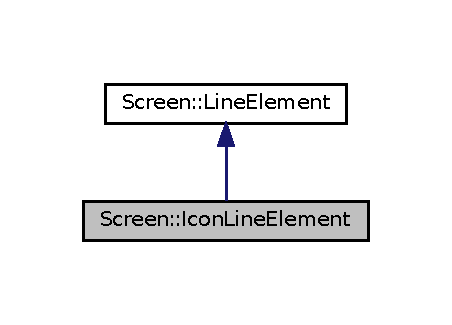
\includegraphics[width=217pt]{classScreen_1_1IconLineElement__inherit__graph}
\end{center}
\end{figure}


Collaboration diagram for Screen\+:\+:Icon\+Line\+Element\+:
\nopagebreak
\begin{figure}[H]
\begin{center}
\leavevmode
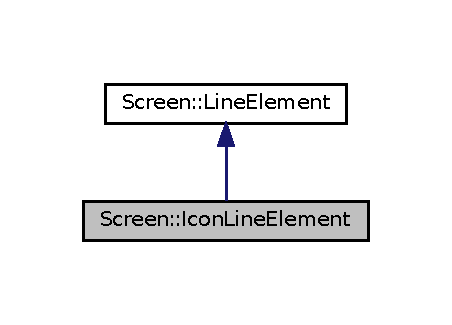
\includegraphics[width=217pt]{classScreen_1_1IconLineElement__coll__graph}
\end{center}
\end{figure}
\subsection*{Public Member Functions}
\begin{DoxyCompactItemize}
\item 
\mbox{\hyperlink{classScreen_1_1IconLineElement_ad465a9f557b9f7e659ebfb8a5a995ca6}{Icon\+Line\+Element}} (uint16\+\_\+t $\ast$\mbox{\hyperlink{classScreen_1_1IconLineElement_ae84108a5bfda7ba013401c067a8c9aca}{p\+Icon}}=N\+U\+LL, int \mbox{\hyperlink{classScreen_1_1IconLineElement_a95ab319fab5abe27266a092fdb75b58e}{scale\+Exponent}}=0, int margin=0, bool \mbox{\hyperlink{classScreen_1_1LineElement_a0c5f4e33c2df1dce8e4e45b90dac1423}{align\+Right}}=false)
\begin{DoxyCompactList}\small\item\em \mbox{\hyperlink{classScreen_1_1IconLineElement}{Icon\+Line\+Element}} constructor. \end{DoxyCompactList}\item 
\mbox{\hyperlink{classScreen_1_1IconLineElement_a7bba2dffbe294ad65c4cda9d7e462bc6}{Icon\+Line\+Element}} (uint16\+\_\+t $\ast$\mbox{\hyperlink{classScreen_1_1IconLineElement_ae84108a5bfda7ba013401c067a8c9aca}{p\+Icon}}, int \mbox{\hyperlink{classScreen_1_1IconLineElement_a95ab319fab5abe27266a092fdb75b58e}{scale\+Exponent}}, int \mbox{\hyperlink{classScreen_1_1LineElement_a9ed23f9510a11334af9be6f53965f7a6}{margin\+Left}}, int \mbox{\hyperlink{classScreen_1_1LineElement_a3a2077f01072be8e8fd0f4539b85beb0}{margin\+Right}}, bool \mbox{\hyperlink{classScreen_1_1LineElement_a0c5f4e33c2df1dce8e4e45b90dac1423}{align\+Right}}=false)
\begin{DoxyCompactList}\small\item\em \mbox{\hyperlink{classScreen_1_1IconLineElement}{Icon\+Line\+Element}} constructor with different margins. \end{DoxyCompactList}\item 
int \mbox{\hyperlink{classScreen_1_1IconLineElement_a3ee090b31ee5061974552be4688d937b}{render\+Self}} (\mbox{\hyperlink{classDisplay}{Display}} $\ast$\mbox{\hyperlink{classScreen_aad713267725e8aa8a8def951a07de641}{display}}, int x, int y)
\begin{DoxyCompactList}\small\item\em Renders itself at position x, y to display. \end{DoxyCompactList}\end{DoxyCompactItemize}
\subsection*{Protected Attributes}
\begin{DoxyCompactItemize}
\item 
\mbox{\Hypertarget{classScreen_1_1IconLineElement_ae84108a5bfda7ba013401c067a8c9aca}\label{classScreen_1_1IconLineElement_ae84108a5bfda7ba013401c067a8c9aca}} 
uint16\+\_\+t $\ast$ \mbox{\hyperlink{classScreen_1_1IconLineElement_ae84108a5bfda7ba013401c067a8c9aca}{p\+Icon}}
\begin{DoxyCompactList}\small\item\em Pointer to the icon buffer. \end{DoxyCompactList}\item 
int \mbox{\hyperlink{classScreen_1_1IconLineElement_a95ab319fab5abe27266a092fdb75b58e}{scale\+Exponent}}
\begin{DoxyCompactList}\small\item\em Exponent to scale icon by. \end{DoxyCompactList}\end{DoxyCompactItemize}
\subsection*{Additional Inherited Members}


\subsection{Detailed Description}
Scaled icon. 

\subsection{Constructor \& Destructor Documentation}
\mbox{\Hypertarget{classScreen_1_1IconLineElement_ad465a9f557b9f7e659ebfb8a5a995ca6}\label{classScreen_1_1IconLineElement_ad465a9f557b9f7e659ebfb8a5a995ca6}} 
\index{Screen\+::\+Icon\+Line\+Element@{Screen\+::\+Icon\+Line\+Element}!Icon\+Line\+Element@{Icon\+Line\+Element}}
\index{Icon\+Line\+Element@{Icon\+Line\+Element}!Screen\+::\+Icon\+Line\+Element@{Screen\+::\+Icon\+Line\+Element}}
\subsubsection{\texorpdfstring{Icon\+Line\+Element()}{IconLineElement()}\hspace{0.1cm}{\footnotesize\ttfamily [1/2]}}
{\footnotesize\ttfamily Screen\+::\+Icon\+Line\+Element\+::\+Icon\+Line\+Element (\begin{DoxyParamCaption}\item[{uint16\+\_\+t $\ast$}]{p\+Icon = {\ttfamily NULL},  }\item[{int}]{scale\+Exponent = {\ttfamily 0},  }\item[{int}]{margin = {\ttfamily 0},  }\item[{bool}]{align\+Right = {\ttfamily false} }\end{DoxyParamCaption})}



\mbox{\hyperlink{classScreen_1_1IconLineElement}{Icon\+Line\+Element}} constructor. 


\begin{DoxyParams}[1]{Parameters}
\mbox{\tt in}  & {\em p\+Icon} & \\
\hline
\mbox{\tt in}  & {\em scale\+Exponent} & \\
\hline
\mbox{\tt in}  & {\em margin} & \\
\hline
\mbox{\tt in}  & {\em align\+Right} & \\
\hline
\end{DoxyParams}
\mbox{\Hypertarget{classScreen_1_1IconLineElement_a7bba2dffbe294ad65c4cda9d7e462bc6}\label{classScreen_1_1IconLineElement_a7bba2dffbe294ad65c4cda9d7e462bc6}} 
\index{Screen\+::\+Icon\+Line\+Element@{Screen\+::\+Icon\+Line\+Element}!Icon\+Line\+Element@{Icon\+Line\+Element}}
\index{Icon\+Line\+Element@{Icon\+Line\+Element}!Screen\+::\+Icon\+Line\+Element@{Screen\+::\+Icon\+Line\+Element}}
\subsubsection{\texorpdfstring{Icon\+Line\+Element()}{IconLineElement()}\hspace{0.1cm}{\footnotesize\ttfamily [2/2]}}
{\footnotesize\ttfamily Screen\+::\+Icon\+Line\+Element\+::\+Icon\+Line\+Element (\begin{DoxyParamCaption}\item[{uint16\+\_\+t $\ast$}]{p\+Icon,  }\item[{int}]{scale\+Exponent,  }\item[{int}]{margin\+Left,  }\item[{int}]{margin\+Right,  }\item[{bool}]{align\+Right = {\ttfamily false} }\end{DoxyParamCaption})}



\mbox{\hyperlink{classScreen_1_1IconLineElement}{Icon\+Line\+Element}} constructor with different margins. 


\begin{DoxyParams}[1]{Parameters}
\mbox{\tt in}  & {\em p\+Icon} & \\
\hline
\mbox{\tt in}  & {\em scale\+Exponent} & \\
\hline
\mbox{\tt in}  & {\em margin\+Left} & \\
\hline
\mbox{\tt in}  & {\em margin\+Right} & \\
\hline
\mbox{\tt in}  & {\em align\+Right} & \\
\hline
\end{DoxyParams}


\subsection{Member Function Documentation}
\mbox{\Hypertarget{classScreen_1_1IconLineElement_a3ee090b31ee5061974552be4688d937b}\label{classScreen_1_1IconLineElement_a3ee090b31ee5061974552be4688d937b}} 
\index{Screen\+::\+Icon\+Line\+Element@{Screen\+::\+Icon\+Line\+Element}!render\+Self@{render\+Self}}
\index{render\+Self@{render\+Self}!Screen\+::\+Icon\+Line\+Element@{Screen\+::\+Icon\+Line\+Element}}
\subsubsection{\texorpdfstring{render\+Self()}{renderSelf()}}
{\footnotesize\ttfamily int Screen\+::\+Icon\+Line\+Element\+::render\+Self (\begin{DoxyParamCaption}\item[{\mbox{\hyperlink{classDisplay}{Display}} $\ast$}]{display,  }\item[{int}]{x,  }\item[{int}]{y }\end{DoxyParamCaption})\hspace{0.3cm}{\ttfamily [virtual]}}



Renders itself at position x, y to display. 


\begin{DoxyParams}[1]{Parameters}
\mbox{\tt in}  & {\em display} & \mbox{\hyperlink{classDisplay}{Display}} to render to. \\
\hline
\mbox{\tt in}  & {\em x} & X position to render to. \\
\hline
\mbox{\tt in}  & {\em y} & Y position to render to. \\
\hline
\end{DoxyParams}
\begin{DoxyReturn}{Returns}
Number of pixels this elements takes. 
\end{DoxyReturn}


Implements \mbox{\hyperlink{classScreen_1_1LineElement_a667fbf6505fbed274ca9a3deac3fef9e}{Screen\+::\+Line\+Element}}.



\subsection{Member Data Documentation}
\mbox{\Hypertarget{classScreen_1_1IconLineElement_a95ab319fab5abe27266a092fdb75b58e}\label{classScreen_1_1IconLineElement_a95ab319fab5abe27266a092fdb75b58e}} 
\index{Screen\+::\+Icon\+Line\+Element@{Screen\+::\+Icon\+Line\+Element}!scale\+Exponent@{scale\+Exponent}}
\index{scale\+Exponent@{scale\+Exponent}!Screen\+::\+Icon\+Line\+Element@{Screen\+::\+Icon\+Line\+Element}}
\subsubsection{\texorpdfstring{scale\+Exponent}{scaleExponent}}
{\footnotesize\ttfamily int Screen\+::\+Icon\+Line\+Element\+::scale\+Exponent\hspace{0.3cm}{\ttfamily [protected]}}



Exponent to scale icon by. 

\begin{DoxySeeAlso}{See also}
\mbox{\hyperlink{classDisplay_a7e1b0ac97b561093e8f1993d7743c095}{Display\+::render\+Icon}} 
\end{DoxySeeAlso}


The documentation for this class was generated from the following files\+:\begin{DoxyCompactItemize}
\item 
Display\+Utils/Screen.\+h\item 
Display\+Utils/Screen.\+cpp\end{DoxyCompactItemize}

\hypertarget{classLightUnit}{}\section{Light\+Unit Class Reference}
\label{classLightUnit}\index{Light\+Unit@{Light\+Unit}}
\subsection*{Public Member Functions}
\begin{DoxyCompactItemize}
\item 
{\bfseries Light\+Unit} (\hyperlink{classLightUnit}{Light\+Unit} \&\&other)\hypertarget{classLightUnit_a171818bc7fbf21a112582ab66c39dedc}{}\label{classLightUnit_a171818bc7fbf21a112582ab66c39dedc}

\item 
{\bfseries Light\+Unit} (const char description\mbox{[}16\mbox{]})\hypertarget{classLightUnit_aa44c2d7b6e764c9bbca0f5ab19a31553}{}\label{classLightUnit_aa44c2d7b6e764c9bbca0f5ab19a31553}

\item 
{\bfseries Light\+Unit} (unsigned long ip, const char description\mbox{[}16\mbox{]}, const uint16\+\_\+t image\mbox{[}256\mbox{]})\hypertarget{classLightUnit_afb696351f25e3766eb18d6ce31f97fa6}{}\label{classLightUnit_afb696351f25e3766eb18d6ce31f97fa6}

\item 
{\bfseries Light\+Unit} (unsigned long ip, const char description\mbox{[}16\mbox{]}, const uint16\+\_\+t image\mbox{[}256\mbox{]}, uint32\+\_\+t rgb\+Ceiling, uint32\+\_\+t rgb\+Wall)\hypertarget{classLightUnit_ab91f948d033d6982b4b981aea104b1d7}{}\label{classLightUnit_ab91f948d033d6982b4b981aea104b1d7}

\item 
\hyperlink{classLightUnit}{Light\+Unit} \& {\bfseries operator=} (\hyperlink{classLightUnit}{Light\+Unit} \&\&other)\hypertarget{classLightUnit_a8c06848d212e79eecdada6751284a484}{}\label{classLightUnit_a8c06848d212e79eecdada6751284a484}

\end{DoxyCompactItemize}
\subsection*{Public Attributes}
\begin{DoxyCompactItemize}
\item 
uint32\+\_\+t {\bfseries rgb\+Ceiling} = 0\hypertarget{classLightUnit_ae688f610193b69a2f390bd2a44dc2a7c}{}\label{classLightUnit_ae688f610193b69a2f390bd2a44dc2a7c}

\item 
uint32\+\_\+t {\bfseries rgb\+Wall} = 0\hypertarget{classLightUnit_a9927e4bcf968e043883688e87935fb4a}{}\label{classLightUnit_a9927e4bcf968e043883688e87935fb4a}

\item 
char {\bfseries description} \mbox{[}17\mbox{]}\hypertarget{classLightUnit_aad36ad5ba65b93a30ee35ef1f6895b5a}{}\label{classLightUnit_aad36ad5ba65b93a30ee35ef1f6895b5a}

\item 
uint16\+\_\+t {\bfseries image} \mbox{[}256\mbox{]}\hypertarget{classLightUnit_a01f65fda0c55ecd8b1d62911cfa688d2}{}\label{classLightUnit_a01f65fda0c55ecd8b1d62911cfa688d2}

\item 
unsigned long {\bfseries ip} = 0\hypertarget{classLightUnit_a7d490bbccb134d200628eee46ab8fb3d}{}\label{classLightUnit_a7d490bbccb134d200628eee46ab8fb3d}

\item 
std\+::chrono\+::steady\+\_\+clock\+::time\+\_\+point {\bfseries last\+Network\+Broadcast\+Time\+Point}\hypertarget{classLightUnit_ac5f86e26fe02c192736cddd1d06af583}{}\label{classLightUnit_ac5f86e26fe02c192736cddd1d06af583}

\item 
std\+::mutex {\bfseries mutex\+\_\+change}\hypertarget{classLightUnit_a4380f5dead3b35443b09f1dbbe44af55}{}\label{classLightUnit_a4380f5dead3b35443b09f1dbbe44af55}

\item 
std\+::atomic$<$ std\+::uint32\+\_\+t $>$ {\bfseries counter\+\_\+readers}\hypertarget{classLightUnit_aba39125324f42994fd370a25aa276de7}{}\label{classLightUnit_aba39125324f42994fd370a25aa276de7}

\end{DoxyCompactItemize}


The documentation for this class was generated from the following files\+:\begin{DoxyCompactItemize}
\item 
Unit/Light\+Unit.\+h\item 
Unit/Light\+Unit.\+cpp\end{DoxyCompactItemize}

\hypertarget{classScreen_1_1LineElement}{}\section{Screen\+:\+:Line\+Element Class Reference}
\label{classScreen_1_1LineElement}\index{Screen\+::\+Line\+Element@{Screen\+::\+Line\+Element}}


Line element base class.  




{\ttfamily \#include $<$Screen.\+h$>$}



Inheritance diagram for Screen\+:\+:Line\+Element\+:
\nopagebreak
\begin{figure}[H]
\begin{center}
\leavevmode
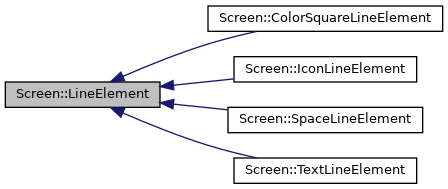
\includegraphics[width=350pt]{classScreen_1_1LineElement__inherit__graph}
\end{center}
\end{figure}
\subsection*{Public Member Functions}
\begin{DoxyCompactItemize}
\item 
\mbox{\hyperlink{classScreen_1_1LineElement_a3f822f160e15ee96022b95026e52ee42}{Line\+Element}} (int margin=0, bool \mbox{\hyperlink{classScreen_1_1LineElement_a0c5f4e33c2df1dce8e4e45b90dac1423}{align\+Right}}=false)
\begin{DoxyCompactList}\small\item\em \mbox{\hyperlink{classScreen_1_1LineElement}{Line\+Element}} constructor. \end{DoxyCompactList}\item 
\mbox{\hyperlink{classScreen_1_1LineElement_a65fe216ee2acbc1191b1fd51b25b2ec7}{Line\+Element}} (int \mbox{\hyperlink{classScreen_1_1LineElement_a9ed23f9510a11334af9be6f53965f7a6}{margin\+Left}}, int \mbox{\hyperlink{classScreen_1_1LineElement_a3a2077f01072be8e8fd0f4539b85beb0}{margin\+Right}}, bool \mbox{\hyperlink{classScreen_1_1LineElement_a0c5f4e33c2df1dce8e4e45b90dac1423}{align\+Right}}=false)
\begin{DoxyCompactList}\small\item\em \mbox{\hyperlink{classScreen_1_1LineElement}{Line\+Element}} constructor with different margins. \end{DoxyCompactList}\item 
virtual int \mbox{\hyperlink{classScreen_1_1LineElement_a667fbf6505fbed274ca9a3deac3fef9e}{render\+Self}} (\mbox{\hyperlink{classDisplay}{Display}} $\ast$\mbox{\hyperlink{classScreen_aad713267725e8aa8a8def951a07de641}{display}}, int x, int y)=0
\begin{DoxyCompactList}\small\item\em Renders itself at position x, y to display. \end{DoxyCompactList}\end{DoxyCompactItemize}
\subsection*{Public Attributes}
\begin{DoxyCompactItemize}
\item 
\mbox{\Hypertarget{classScreen_1_1LineElement_a0c5f4e33c2df1dce8e4e45b90dac1423}\label{classScreen_1_1LineElement_a0c5f4e33c2df1dce8e4e45b90dac1423}} 
bool \mbox{\hyperlink{classScreen_1_1LineElement_a0c5f4e33c2df1dce8e4e45b90dac1423}{align\+Right}}
\begin{DoxyCompactList}\small\item\em Wether to align left or right. \end{DoxyCompactList}\end{DoxyCompactItemize}
\subsection*{Protected Attributes}
\begin{DoxyCompactItemize}
\item 
\mbox{\Hypertarget{classScreen_1_1LineElement_a9ed23f9510a11334af9be6f53965f7a6}\label{classScreen_1_1LineElement_a9ed23f9510a11334af9be6f53965f7a6}} 
int \mbox{\hyperlink{classScreen_1_1LineElement_a9ed23f9510a11334af9be6f53965f7a6}{margin\+Left}}
\begin{DoxyCompactList}\small\item\em Left margin of this element. Can be negative. \end{DoxyCompactList}\item 
\mbox{\Hypertarget{classScreen_1_1LineElement_a3a2077f01072be8e8fd0f4539b85beb0}\label{classScreen_1_1LineElement_a3a2077f01072be8e8fd0f4539b85beb0}} 
int \mbox{\hyperlink{classScreen_1_1LineElement_a3a2077f01072be8e8fd0f4539b85beb0}{margin\+Right}}
\begin{DoxyCompactList}\small\item\em Right margin of this element. Can be negative. \end{DoxyCompactList}\end{DoxyCompactItemize}


\subsection{Detailed Description}
Line element base class. 

\subsection{Constructor \& Destructor Documentation}
\mbox{\Hypertarget{classScreen_1_1LineElement_a3f822f160e15ee96022b95026e52ee42}\label{classScreen_1_1LineElement_a3f822f160e15ee96022b95026e52ee42}} 
\index{Screen\+::\+Line\+Element@{Screen\+::\+Line\+Element}!Line\+Element@{Line\+Element}}
\index{Line\+Element@{Line\+Element}!Screen\+::\+Line\+Element@{Screen\+::\+Line\+Element}}
\subsubsection{\texorpdfstring{Line\+Element()}{LineElement()}\hspace{0.1cm}{\footnotesize\ttfamily [1/2]}}
{\footnotesize\ttfamily Screen\+::\+Line\+Element\+::\+Line\+Element (\begin{DoxyParamCaption}\item[{int}]{margin = {\ttfamily 0},  }\item[{bool}]{align\+Right = {\ttfamily false} }\end{DoxyParamCaption})}



\mbox{\hyperlink{classScreen_1_1LineElement}{Line\+Element}} constructor. 


\begin{DoxyParams}[1]{Parameters}
\mbox{\tt in}  & {\em margin} & \\
\hline
\mbox{\tt in}  & {\em align\+Right} & \\
\hline
\end{DoxyParams}
\mbox{\Hypertarget{classScreen_1_1LineElement_a65fe216ee2acbc1191b1fd51b25b2ec7}\label{classScreen_1_1LineElement_a65fe216ee2acbc1191b1fd51b25b2ec7}} 
\index{Screen\+::\+Line\+Element@{Screen\+::\+Line\+Element}!Line\+Element@{Line\+Element}}
\index{Line\+Element@{Line\+Element}!Screen\+::\+Line\+Element@{Screen\+::\+Line\+Element}}
\subsubsection{\texorpdfstring{Line\+Element()}{LineElement()}\hspace{0.1cm}{\footnotesize\ttfamily [2/2]}}
{\footnotesize\ttfamily Screen\+::\+Line\+Element\+::\+Line\+Element (\begin{DoxyParamCaption}\item[{int}]{margin\+Left,  }\item[{int}]{margin\+Right,  }\item[{bool}]{align\+Right = {\ttfamily false} }\end{DoxyParamCaption})}



\mbox{\hyperlink{classScreen_1_1LineElement}{Line\+Element}} constructor with different margins. 


\begin{DoxyParams}[1]{Parameters}
\mbox{\tt in}  & {\em margin\+Left} & \\
\hline
\mbox{\tt in}  & {\em margin\+Right} & \\
\hline
\mbox{\tt in}  & {\em align\+Right} & \\
\hline
\end{DoxyParams}


\subsection{Member Function Documentation}
\mbox{\Hypertarget{classScreen_1_1LineElement_a667fbf6505fbed274ca9a3deac3fef9e}\label{classScreen_1_1LineElement_a667fbf6505fbed274ca9a3deac3fef9e}} 
\index{Screen\+::\+Line\+Element@{Screen\+::\+Line\+Element}!render\+Self@{render\+Self}}
\index{render\+Self@{render\+Self}!Screen\+::\+Line\+Element@{Screen\+::\+Line\+Element}}
\subsubsection{\texorpdfstring{render\+Self()}{renderSelf()}}
{\footnotesize\ttfamily virtual int Screen\+::\+Line\+Element\+::render\+Self (\begin{DoxyParamCaption}\item[{\mbox{\hyperlink{classDisplay}{Display}} $\ast$}]{display,  }\item[{int}]{x,  }\item[{int}]{y }\end{DoxyParamCaption})\hspace{0.3cm}{\ttfamily [pure virtual]}}



Renders itself at position x, y to display. 


\begin{DoxyParams}[1]{Parameters}
\mbox{\tt in}  & {\em display} & \mbox{\hyperlink{classDisplay}{Display}} to render to. \\
\hline
\mbox{\tt in}  & {\em x} & X position to render to. \\
\hline
\mbox{\tt in}  & {\em y} & Y position to render to. \\
\hline
\end{DoxyParams}
\begin{DoxyReturn}{Returns}
Number of pixels this elements takes. 
\end{DoxyReturn}


Implemented in \mbox{\hyperlink{classScreen_1_1IconLineElement_a3ee090b31ee5061974552be4688d937b}{Screen\+::\+Icon\+Line\+Element}}, \mbox{\hyperlink{classScreen_1_1TextLineElement_abcd2e0700f84bb19d7a285345cd37871}{Screen\+::\+Text\+Line\+Element}}, \mbox{\hyperlink{classScreen_1_1ColorSquareLineElement_abea938100788da99f8ded53ca642edc0}{Screen\+::\+Color\+Square\+Line\+Element}}, and \mbox{\hyperlink{classScreen_1_1SpaceLineElement_a897336996ddbfbb7c86bb6ef9acb8536}{Screen\+::\+Space\+Line\+Element}}.



The documentation for this class was generated from the following files\+:\begin{DoxyCompactItemize}
\item 
Display\+Utils/Screen.\+h\item 
Display\+Utils/Screen.\+cpp\end{DoxyCompactItemize}

\hypertarget{classListScreen}{}\section{List\+Screen Class Reference}
\label{classListScreen}\index{List\+Screen@{List\+Screen}}


Unit screen.  




{\ttfamily \#include $<$List\+Screen.\+h$>$}



Inheritance diagram for List\+Screen\+:\nopagebreak
\begin{figure}[H]
\begin{center}
\leavevmode
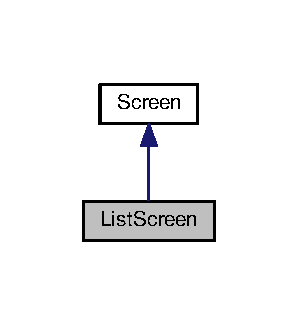
\includegraphics[width=143pt]{classListScreen__inherit__graph}
\end{center}
\end{figure}


Collaboration diagram for List\+Screen\+:\nopagebreak
\begin{figure}[H]
\begin{center}
\leavevmode
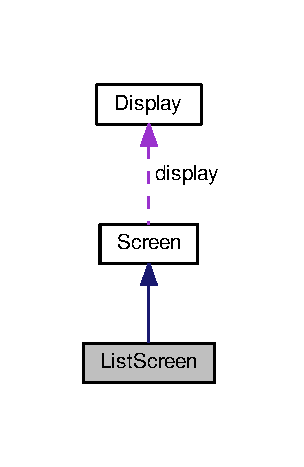
\includegraphics[width=146pt]{classListScreen__coll__graph}
\end{center}
\end{figure}
\subsection*{Public Member Functions}
\begin{DoxyCompactItemize}
\item 
\mbox{\Hypertarget{classListScreen_a502ff7cf893ae6d10ed7bc1ca7a8ffe8}\label{classListScreen_a502ff7cf893ae6d10ed7bc1ca7a8ffe8}} 
{\bfseries List\+Screen} (\mbox{\hyperlink{classDisplay}{Display}} $\ast$display)
\item 
\mbox{\Hypertarget{classListScreen_a364b4ccc88650c13295efae8431b135e}\label{classListScreen_a364b4ccc88650c13295efae8431b135e}} 
void \mbox{\hyperlink{classListScreen_a364b4ccc88650c13295efae8431b135e}{render\+Screen}} ()
\begin{DoxyCompactList}\small\item\em Renders this screen to display. \end{DoxyCompactList}\item 
\mbox{\Hypertarget{classListScreen_a4e0f2e67dbfbcf8560209f01d2cab1c6}\label{classListScreen_a4e0f2e67dbfbcf8560209f01d2cab1c6}} 
void \mbox{\hyperlink{classListScreen_a4e0f2e67dbfbcf8560209f01d2cab1c6}{handle\+Knob\+Change}} (int8\+\_\+t R\+G\+B\+Delta\mbox{[}3\mbox{]})
\begin{DoxyCompactList}\small\item\em Handles knob changes. \end{DoxyCompactList}\item 
\mbox{\Hypertarget{classListScreen_aecf861357be2b6debde43e61c9a7671b}\label{classListScreen_aecf861357be2b6debde43e61c9a7671b}} 
void \mbox{\hyperlink{classListScreen_aecf861357be2b6debde43e61c9a7671b}{handle\+Knob\+Press}} (bool R\+G\+B\+Pressed\mbox{[}3\mbox{]})
\begin{DoxyCompactList}\small\item\em Handles knob presses. \end{DoxyCompactList}\end{DoxyCompactItemize}
\subsection*{Additional Inherited Members}


\subsection{Detailed Description}
Unit screen. 

This screen renders list of all connected units and allows selection to pass to Unit screen. \begin{DoxySeeAlso}{See also}
\mbox{\hyperlink{classUnitScreen}{Unit\+Screen}} 
\end{DoxySeeAlso}


The documentation for this class was generated from the following files\+:\begin{DoxyCompactItemize}
\item 
Display\+Utils/List\+Screen.\+h\item 
Display\+Utils/List\+Screen.\+cpp\end{DoxyCompactItemize}

\hypertarget{classMapper}{}\section{Mapper Class Reference}
\label{classMapper}\index{Mapper@{Mapper}}


{\ttfamily \#include $<$Mapper.\+h$>$}

\subsection*{Public Member Functions}
\begin{DoxyCompactItemize}
\item 
\mbox{\hyperlink{classMapper_ad94bc5276f51985b51f72922f64bc19e}{Mapper}} (off\+\_\+t base, size\+\_\+t size)
\end{DoxyCompactItemize}
\subsection*{Public Attributes}
\begin{DoxyCompactItemize}
\item 
\mbox{\Hypertarget{classMapper_afadadee19eb92436827f4f1e8c71a4e6}\label{classMapper_afadadee19eb92436827f4f1e8c71a4e6}} 
unsigned char $\ast$ {\bfseries mem\+\_\+base} = N\+U\+LL
\end{DoxyCompactItemize}


\subsection{Detailed Description}
A class that handles the mapping of peripheral physical regions to virtual addresses. 

\subsection{Constructor \& Destructor Documentation}
\mbox{\Hypertarget{classMapper_ad94bc5276f51985b51f72922f64bc19e}\label{classMapper_ad94bc5276f51985b51f72922f64bc19e}} 
\index{Mapper@{Mapper}!Mapper@{Mapper}}
\index{Mapper@{Mapper}!Mapper@{Mapper}}
\subsubsection{\texorpdfstring{Mapper()}{Mapper()}}
{\footnotesize\ttfamily Mapper\+::\+Mapper (\begin{DoxyParamCaption}\item[{off\+\_\+t}]{base,  }\item[{size\+\_\+t}]{size }\end{DoxyParamCaption})}

Constructor for \mbox{\hyperlink{classMapper}{Mapper}}. 
\begin{DoxyParams}{Parameters}
{\em base} & The base region of the peripheral. \\
\hline
{\em size} & Address range for the region. \\
\hline
\end{DoxyParams}


The documentation for this class was generated from the following files\+:\begin{DoxyCompactItemize}
\item 
M\+Z\+Api/Mapper.\+h\item 
M\+Z\+Api/Mapper.\+cpp\end{DoxyCompactItemize}

\hypertarget{structNetworkHandler_1_1Message}{}\section{Network\+Handler\+:\+:Message Struct Reference}
\label{structNetworkHandler_1_1Message}\index{Network\+Handler\+::\+Message@{Network\+Handler\+::\+Message}}


Inheritance diagram for Network\+Handler\+:\+:Message\+:\nopagebreak
\begin{figure}[H]
\begin{center}
\leavevmode
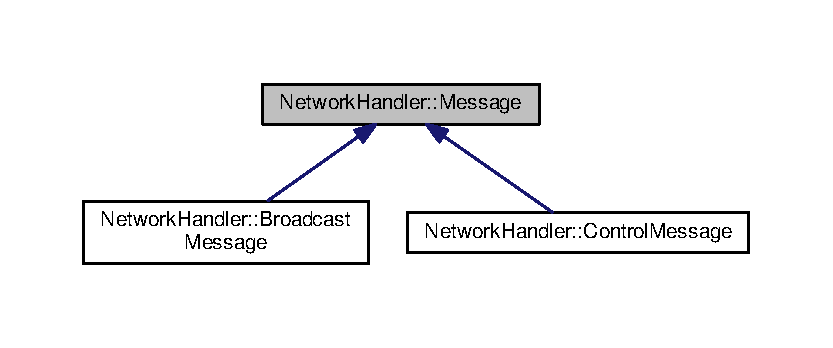
\includegraphics[width=350pt]{structNetworkHandler_1_1Message__inherit__graph}
\end{center}
\end{figure}
\subsection*{Public Attributes}
\begin{DoxyCompactItemize}
\item 
uint32\+\_\+t {\bfseries magic}\hypertarget{structNetworkHandler_1_1Message_a223522c0b8a50767dd4440998a723ce8}{}\label{structNetworkHandler_1_1Message_a223522c0b8a50767dd4440998a723ce8}

\item 
uint32\+\_\+t {\bfseries version}\hypertarget{structNetworkHandler_1_1Message_a806b0186d262219408b53c7137489034}{}\label{structNetworkHandler_1_1Message_a806b0186d262219408b53c7137489034}

\item 
uint32\+\_\+t {\bfseries msg\+Type}\hypertarget{structNetworkHandler_1_1Message_a3a05df44411cb9ac7c8a7842a5afbff4}{}\label{structNetworkHandler_1_1Message_a3a05df44411cb9ac7c8a7842a5afbff4}

\end{DoxyCompactItemize}


The documentation for this struct was generated from the following file\+:\begin{DoxyCompactItemize}
\item 
Network/Network\+Handler.\+h\end{DoxyCompactItemize}

\hypertarget{classNetworkHandler}{}\section{Network\+Handler Class Reference}
\label{classNetworkHandler}\index{Network\+Handler@{Network\+Handler}}
\subsection*{Classes}
\begin{DoxyCompactItemize}
\item 
struct \hyperlink{structNetworkHandler_1_1BroadcastMessage}{Broadcast\+Message}
\item 
struct \hyperlink{structNetworkHandler_1_1ControlMessage}{Control\+Message}
\item 
struct \hyperlink{structNetworkHandler_1_1Message}{Message}
\item 
struct \hyperlink{structNetworkHandler_1_1RecievedMessage}{Recieved\+Message}
\end{DoxyCompactItemize}
\subsection*{Public Types}
\begin{DoxyCompactItemize}
\item 
typedef struct \hyperlink{structNetworkHandler_1_1Message}{Network\+Handler\+::\+Message} {\bfseries Message}\hypertarget{classNetworkHandler_a40a384ea43787b06682a000b015add29}{}\label{classNetworkHandler_a40a384ea43787b06682a000b015add29}

\item 
typedef \hyperlink{structNetworkHandler_1_1BroadcastMessage}{Network\+Handler\+::\+Broadcast\+Message} {\bfseries Broadcast\+Message}\hypertarget{classNetworkHandler_a5efffc9f48abe8087c6f756e33d5eb9e}{}\label{classNetworkHandler_a5efffc9f48abe8087c6f756e33d5eb9e}

\item 
typedef \hyperlink{structNetworkHandler_1_1ControlMessage}{Network\+Handler\+::\+Control\+Message} {\bfseries Control\+Message}\hypertarget{classNetworkHandler_a29cb429e8069fa3c00b8317aec0b735a}{}\label{classNetworkHandler_a29cb429e8069fa3c00b8317aec0b735a}

\item 
typedef struct \hyperlink{structNetworkHandler_1_1RecievedMessage}{Network\+Handler\+::\+Recieved\+Message} {\bfseries Recieved\+Message}\hypertarget{classNetworkHandler_a558eabe1d275787ab92e63c7bbabf19c}{}\label{classNetworkHandler_a558eabe1d275787ab92e63c7bbabf19c}

\end{DoxyCompactItemize}
\subsection*{Public Member Functions}
\begin{DoxyCompactItemize}
\item 
bool {\bfseries broadcast\+Message} (const \hyperlink{structNetworkHandler_1_1BroadcastMessage}{Broadcast\+Message} $\ast$message)\hypertarget{classNetworkHandler_a3296b0356692982086aacad3f34b7c12}{}\label{classNetworkHandler_a3296b0356692982086aacad3f34b7c12}

\item 
bool {\bfseries broadcast\+Unit} (\hyperlink{classLightUnit}{Light\+Unit} \&unit)\hypertarget{classNetworkHandler_a515ae3ef779f2244cfdcccbbb24c8cb2}{}\label{classNetworkHandler_a515ae3ef779f2244cfdcccbbb24c8cb2}

\item 
bool {\bfseries send\+Message} (const \hyperlink{structNetworkHandler_1_1ControlMessage}{Control\+Message} $\ast$message, uint32\+\_\+t ip)\hypertarget{classNetworkHandler_ae424a6a062dd0244560908d8de1798d0}{}\label{classNetworkHandler_ae424a6a062dd0244560908d8de1798d0}

\item 
\hyperlink{structNetworkHandler_1_1BroadcastMessage}{Broadcast\+Message} {\bfseries build\+Broadcast\+Message} (\hyperlink{classLightUnit}{Light\+Unit} \&unit)\hypertarget{classNetworkHandler_a0e8984b42f72b35466d409319c938e4d}{}\label{classNetworkHandler_a0e8984b42f72b35466d409319c938e4d}

\item 
\hyperlink{structNetworkHandler_1_1ControlMessage}{Control\+Message} {\bfseries build\+Control\+Message} (int type, int16\+\_\+t values\+Ceiling\mbox{[}$\,$\mbox{]}, int16\+\_\+t values\+Wall\mbox{[}$\,$\mbox{]})\hypertarget{classNetworkHandler_ac43127d9c50aeba5c9bbc853bef447a9}{}\label{classNetworkHandler_ac43127d9c50aeba5c9bbc853bef447a9}

\item 
\hyperlink{structNetworkHandler_1_1RecievedMessage}{Recieved\+Message} {\bfseries recieve\+Message} ()\hypertarget{classNetworkHandler_a0c605f9d3c9ae3d7d55c1edffdba7d84}{}\label{classNetworkHandler_a0c605f9d3c9ae3d7d55c1edffdba7d84}

\end{DoxyCompactItemize}


The documentation for this class was generated from the following files\+:\begin{DoxyCompactItemize}
\item 
Network/Network\+Handler.\+h\item 
Network/Network\+Handler.\+cpp\end{DoxyCompactItemize}

\hypertarget{classNyanScreen}{}\section{Nyan\+Screen Class Reference}
\label{classNyanScreen}\index{Nyan\+Screen@{Nyan\+Screen}}


Inheritance diagram for Nyan\+Screen\+:\nopagebreak
\begin{figure}[H]
\begin{center}
\leavevmode
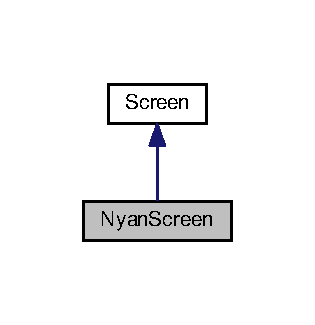
\includegraphics[width=151pt]{classNyanScreen__inherit__graph}
\end{center}
\end{figure}


Collaboration diagram for Nyan\+Screen\+:\nopagebreak
\begin{figure}[H]
\begin{center}
\leavevmode
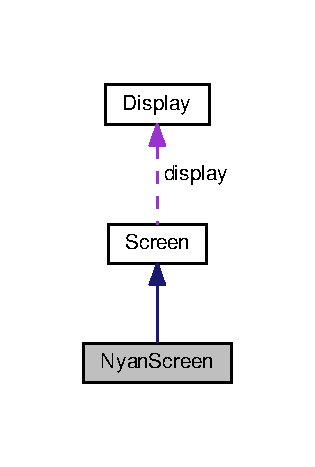
\includegraphics[width=151pt]{classNyanScreen__coll__graph}
\end{center}
\end{figure}
\subsection*{Public Member Functions}
\begin{DoxyCompactItemize}
\item 
{\bfseries Nyan\+Screen} (\hyperlink{classDisplay}{Display} $\ast$display)\hypertarget{classNyanScreen_acd188f631e8e0ce657b31b94a1fcaed0}{}\label{classNyanScreen_acd188f631e8e0ce657b31b94a1fcaed0}

\item 
void {\bfseries render\+Screen} ()\hypertarget{classNyanScreen_aae9641b13b885eab16ae3bc9e91dee36}{}\label{classNyanScreen_aae9641b13b885eab16ae3bc9e91dee36}

\item 
void {\bfseries handle\+Knob\+Change} (int8\+\_\+t R\+G\+B\+Delta\mbox{[}3\mbox{]})\hypertarget{classNyanScreen_a7fc740bda8f8a3147565433264f4bb4f}{}\label{classNyanScreen_a7fc740bda8f8a3147565433264f4bb4f}

\item 
void {\bfseries handle\+Knob\+Press} (bool R\+G\+B\+Pressed\mbox{[}3\mbox{]})\hypertarget{classNyanScreen_a5c59bde088c7e56a616c99cd51f6ab82}{}\label{classNyanScreen_a5c59bde088c7e56a616c99cd51f6ab82}

\end{DoxyCompactItemize}
\subsection*{Additional Inherited Members}


The documentation for this class was generated from the following files\+:\begin{DoxyCompactItemize}
\item 
Display\+Utils/Nyan\+Screen.\+h\item 
Display\+Utils/Nyan\+Screen.\+cpp\end{DoxyCompactItemize}

\hypertarget{structNetworkHandler_1_1RecievedMessage}{}\section{Network\+Handler\+:\+:Recieved\+Message Struct Reference}
\label{structNetworkHandler_1_1RecievedMessage}\index{Network\+Handler\+::\+Recieved\+Message@{Network\+Handler\+::\+Recieved\+Message}}


Collaboration diagram for Network\+Handler\+:\+:Recieved\+Message\+:\nopagebreak
\begin{figure}[H]
\begin{center}
\leavevmode
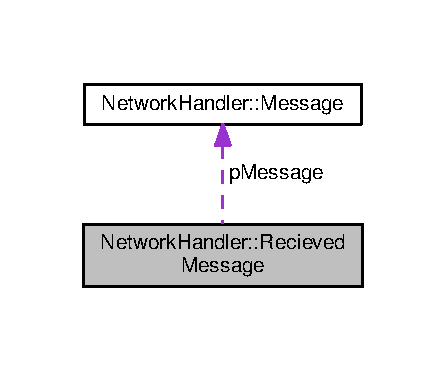
\includegraphics[width=214pt]{structNetworkHandler_1_1RecievedMessage__coll__graph}
\end{center}
\end{figure}
\subsection*{Public Attributes}
\begin{DoxyCompactItemize}
\item 
uint32\+\_\+t {\bfseries ip}\hypertarget{structNetworkHandler_1_1RecievedMessage_a6f01f4a042b9f5a4cd40d441e0e29d48}{}\label{structNetworkHandler_1_1RecievedMessage_a6f01f4a042b9f5a4cd40d441e0e29d48}

\item 
std\+::chrono\+::steady\+\_\+clock\+::time\+\_\+point {\bfseries time\+Point}\hypertarget{structNetworkHandler_1_1RecievedMessage_a0ce3474866ebd9fefaeba2cf901959e2}{}\label{structNetworkHandler_1_1RecievedMessage_a0ce3474866ebd9fefaeba2cf901959e2}

\item 
\hyperlink{structNetworkHandler_1_1Message}{Message} $\ast$ {\bfseries p\+Message}\hypertarget{structNetworkHandler_1_1RecievedMessage_a3407eb8d41737f5ab7fbf73fa6813342}{}\label{structNetworkHandler_1_1RecievedMessage_a3407eb8d41737f5ab7fbf73fa6813342}

\end{DoxyCompactItemize}


The documentation for this struct was generated from the following file\+:\begin{DoxyCompactItemize}
\item 
Network/Network\+Handler.\+h\end{DoxyCompactItemize}

\hypertarget{classRWMutex}{}\section{R\+W\+Mutex Class Reference}
\label{classRWMutex}\index{R\+W\+Mutex@{R\+W\+Mutex}}
\subsection*{Public Member Functions}
\begin{DoxyCompactItemize}
\item 
\mbox{\Hypertarget{classRWMutex_ab76f003469059259e2a48e9ed6643c25}\label{classRWMutex_ab76f003469059259e2a48e9ed6643c25}} 
void {\bfseries lock\+Read} ()
\item 
\mbox{\Hypertarget{classRWMutex_aa71e2ce4d243c3d4c471a7fe55381b2f}\label{classRWMutex_aa71e2ce4d243c3d4c471a7fe55381b2f}} 
void {\bfseries unlock\+Read} ()
\item 
\mbox{\Hypertarget{classRWMutex_ac977d0b492c040e36a77b55ee3ae9c04}\label{classRWMutex_ac977d0b492c040e36a77b55ee3ae9c04}} 
void {\bfseries lock\+Write} ()
\item 
\mbox{\Hypertarget{classRWMutex_a2f145529b60c90b3eba0ac0fd547f2b2}\label{classRWMutex_a2f145529b60c90b3eba0ac0fd547f2b2}} 
void {\bfseries unlock\+Write} ()
\end{DoxyCompactItemize}


The documentation for this class was generated from the following files\+:\begin{DoxyCompactItemize}
\item 
Misc/R\+W\+Mutex.\+h\item 
Misc/R\+W\+Mutex.\+cpp\end{DoxyCompactItemize}

\hypertarget{classScreen}{}\section{Screen Class Reference}
\label{classScreen}\index{Screen@{Screen}}


Class representing one screen.  




{\ttfamily \#include $<$Screen.\+h$>$}



Inheritance diagram for Screen\+:\nopagebreak
\begin{figure}[H]
\begin{center}
\leavevmode
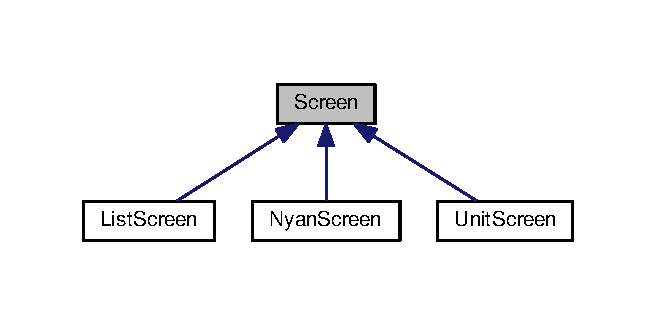
\includegraphics[width=315pt]{classScreen__inherit__graph}
\end{center}
\end{figure}


Collaboration diagram for Screen\+:\nopagebreak
\begin{figure}[H]
\begin{center}
\leavevmode
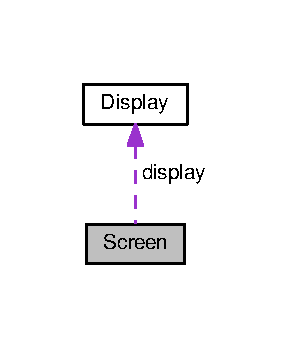
\includegraphics[width=139pt]{classScreen__coll__graph}
\end{center}
\end{figure}
\subsection*{Classes}
\begin{DoxyCompactItemize}
\item 
class \mbox{\hyperlink{classScreen_1_1ColorSquareLineElement}{Color\+Square\+Line\+Element}}
\begin{DoxyCompactList}\small\item\em Color square. \end{DoxyCompactList}\item 
class \mbox{\hyperlink{classScreen_1_1IconLineElement}{Icon\+Line\+Element}}
\begin{DoxyCompactList}\small\item\em Scaled icon. \end{DoxyCompactList}\item 
class \mbox{\hyperlink{classScreen_1_1LineElement}{Line\+Element}}
\begin{DoxyCompactList}\small\item\em Line element base class. \end{DoxyCompactList}\item 
class \mbox{\hyperlink{classScreen_1_1SpaceLineElement}{Space\+Line\+Element}}
\begin{DoxyCompactList}\small\item\em Empty space. \end{DoxyCompactList}\item 
class \mbox{\hyperlink{classScreen_1_1TextLineElement}{Text\+Line\+Element}}
\begin{DoxyCompactList}\small\item\em Text. \end{DoxyCompactList}\end{DoxyCompactItemize}
\subsection*{Public Member Functions}
\begin{DoxyCompactItemize}
\item 
\mbox{\Hypertarget{classScreen_afd1cb4a4bfbbec56cc64c973a9242110}\label{classScreen_afd1cb4a4bfbbec56cc64c973a9242110}} 
virtual void \mbox{\hyperlink{classScreen_afd1cb4a4bfbbec56cc64c973a9242110}{render\+Screen}} ()=0
\begin{DoxyCompactList}\small\item\em Renders this screen to display. \end{DoxyCompactList}\item 
\mbox{\Hypertarget{classScreen_a4c3869a19704ec2530a377618b3f6104}\label{classScreen_a4c3869a19704ec2530a377618b3f6104}} 
virtual void \mbox{\hyperlink{classScreen_a4c3869a19704ec2530a377618b3f6104}{handle\+Knob\+Change}} (int8\+\_\+t R\+G\+B\+Delta\mbox{[}3\mbox{]})=0
\begin{DoxyCompactList}\small\item\em Handles knob changes. \end{DoxyCompactList}\item 
\mbox{\Hypertarget{classScreen_a1b9547f8f48c3ceae2024b58e0746e94}\label{classScreen_a1b9547f8f48c3ceae2024b58e0746e94}} 
virtual void \mbox{\hyperlink{classScreen_a1b9547f8f48c3ceae2024b58e0746e94}{handle\+Knob\+Press}} (bool R\+G\+B\+Pressed\mbox{[}3\mbox{]})=0
\begin{DoxyCompactList}\small\item\em Handles knob presses. \end{DoxyCompactList}\end{DoxyCompactItemize}
\subsection*{Protected Types}
\begin{DoxyCompactItemize}
\item 
\mbox{\Hypertarget{classScreen_a3696376a0036dc304d337dc5e697d6f9}\label{classScreen_a3696376a0036dc304d337dc5e697d6f9}} 
typedef std\+::unique\+\_\+ptr$<$ \mbox{\hyperlink{classScreen_1_1LineElement}{Line\+Element}} $>$ \mbox{\hyperlink{classScreen_a3696376a0036dc304d337dc5e697d6f9}{P\+Line\+Element}}
\begin{DoxyCompactList}\small\item\em One line element pointer. \end{DoxyCompactList}\item 
\mbox{\Hypertarget{classScreen_a62e857d5d7fcfd58fe241c1e933ac3bb}\label{classScreen_a62e857d5d7fcfd58fe241c1e933ac3bb}} 
typedef std\+::vector$<$ \mbox{\hyperlink{classScreen_a3696376a0036dc304d337dc5e697d6f9}{Screen\+::\+P\+Line\+Element}} $>$ \mbox{\hyperlink{classScreen_a62e857d5d7fcfd58fe241c1e933ac3bb}{P\+Line\+Element\+Vector}}
\begin{DoxyCompactList}\small\item\em Vector of line element pointers. \end{DoxyCompactList}\end{DoxyCompactItemize}
\subsection*{Protected Member Functions}
\begin{DoxyCompactItemize}
\item 
\mbox{\hyperlink{classScreen_a596e7fffdfafd57fb5385c299863f31d}{Screen}} (\mbox{\hyperlink{classDisplay}{Display}} $\ast$\mbox{\hyperlink{classScreen_aad713267725e8aa8a8def951a07de641}{display}})
\begin{DoxyCompactList}\small\item\em Creates \mbox{\hyperlink{classScreen}{Screen}} and binds it to display. \end{DoxyCompactList}\item 
void \mbox{\hyperlink{classScreen_a30226bc0c228db9f74f337af86cf34ed}{render\+Line}} (int y, \mbox{\hyperlink{classScreen_a3696376a0036dc304d337dc5e697d6f9}{Screen\+::\+P\+Line\+Element}} element, int32\+\_\+t line\+Color=-\/1)
\begin{DoxyCompactList}\small\item\em Renders line containing only one element. \end{DoxyCompactList}\item 
void \mbox{\hyperlink{classScreen_a21262307ae7898dfa1b27bb0c60247b7}{render\+Line}} (int y, \mbox{\hyperlink{classScreen_a62e857d5d7fcfd58fe241c1e933ac3bb}{Screen\+::\+P\+Line\+Element\+Vector}} \&elements, int32\+\_\+t line\+Color=-\/1)
\begin{DoxyCompactList}\small\item\em Renders line containing elements. \end{DoxyCompactList}\item 
void \mbox{\hyperlink{classScreen_a435b179ec61ea7ad8126102a00051b88}{render\+Nagivation\+Line}} (std\+::vector$<$ std\+::pair$<$ std\+::string, std\+::string $>$$>$ ui\+Input\+Pairs)
\begin{DoxyCompactList}\small\item\em Renders navigation line. \end{DoxyCompactList}\end{DoxyCompactItemize}
\subsection*{Protected Attributes}
\begin{DoxyCompactItemize}
\item 
\mbox{\Hypertarget{classScreen_aad713267725e8aa8a8def951a07de641}\label{classScreen_aad713267725e8aa8a8def951a07de641}} 
\mbox{\hyperlink{classDisplay}{Display}} $\ast$ \mbox{\hyperlink{classScreen_aad713267725e8aa8a8def951a07de641}{display}}
\begin{DoxyCompactList}\small\item\em \mbox{\hyperlink{classDisplay}{Display}} this screen is bound to. \end{DoxyCompactList}\item 
\mbox{\Hypertarget{classScreen_ae66538a4cf9fd681495f28acb12be732}\label{classScreen_ae66538a4cf9fd681495f28acb12be732}} 
size\+\_\+t \mbox{\hyperlink{classScreen_ae66538a4cf9fd681495f28acb12be732}{selected}} = 0
\begin{DoxyCompactList}\small\item\em Currently selected line. \end{DoxyCompactList}\end{DoxyCompactItemize}


\subsection{Detailed Description}
Class representing one screen. 

\subsection{Constructor \& Destructor Documentation}
\mbox{\Hypertarget{classScreen_a596e7fffdfafd57fb5385c299863f31d}\label{classScreen_a596e7fffdfafd57fb5385c299863f31d}} 
\index{Screen@{Screen}!Screen@{Screen}}
\index{Screen@{Screen}!Screen@{Screen}}
\subsubsection{\texorpdfstring{Screen()}{Screen()}}
{\footnotesize\ttfamily Screen\+::\+Screen (\begin{DoxyParamCaption}\item[{\mbox{\hyperlink{classDisplay}{Display}} $\ast$}]{display }\end{DoxyParamCaption})\hspace{0.3cm}{\ttfamily [protected]}}



Creates \mbox{\hyperlink{classScreen}{Screen}} and binds it to display. 


\begin{DoxyParams}[1]{Parameters}
\mbox{\tt in}  & {\em display} & \\
\hline
\end{DoxyParams}


\subsection{Member Function Documentation}
\mbox{\Hypertarget{classScreen_a30226bc0c228db9f74f337af86cf34ed}\label{classScreen_a30226bc0c228db9f74f337af86cf34ed}} 
\index{Screen@{Screen}!render\+Line@{render\+Line}}
\index{render\+Line@{render\+Line}!Screen@{Screen}}
\subsubsection{\texorpdfstring{render\+Line()}{renderLine()}\hspace{0.1cm}{\footnotesize\ttfamily [1/2]}}
{\footnotesize\ttfamily void Screen\+::render\+Line (\begin{DoxyParamCaption}\item[{int}]{y,  }\item[{\mbox{\hyperlink{classScreen_a3696376a0036dc304d337dc5e697d6f9}{Screen\+::\+P\+Line\+Element}}}]{element,  }\item[{int32\+\_\+t}]{line\+Color = {\ttfamily -\/1} }\end{DoxyParamCaption})\hspace{0.3cm}{\ttfamily [protected]}}



Renders line containing only one element. 


\begin{DoxyParams}[1]{Parameters}
\mbox{\tt in}  & {\em y} & Y position to render the line at. \\
\hline
\mbox{\tt in}  & {\em element} & Element to render in this line. \\
\hline
\mbox{\tt in}  & {\em line\+Color} & Color of this line. Pass -\/1 to not draw any line background. \\
\hline
\end{DoxyParams}
\mbox{\Hypertarget{classScreen_a21262307ae7898dfa1b27bb0c60247b7}\label{classScreen_a21262307ae7898dfa1b27bb0c60247b7}} 
\index{Screen@{Screen}!render\+Line@{render\+Line}}
\index{render\+Line@{render\+Line}!Screen@{Screen}}
\subsubsection{\texorpdfstring{render\+Line()}{renderLine()}\hspace{0.1cm}{\footnotesize\ttfamily [2/2]}}
{\footnotesize\ttfamily void Screen\+::render\+Line (\begin{DoxyParamCaption}\item[{int}]{y,  }\item[{\mbox{\hyperlink{classScreen_a62e857d5d7fcfd58fe241c1e933ac3bb}{Screen\+::\+P\+Line\+Element\+Vector}} \&}]{elements,  }\item[{int32\+\_\+t}]{line\+Color = {\ttfamily -\/1} }\end{DoxyParamCaption})\hspace{0.3cm}{\ttfamily [protected]}}



Renders line containing elements. 


\begin{DoxyParams}[1]{Parameters}
\mbox{\tt in}  & {\em y} & Y position to render the line at. \\
\hline
\mbox{\tt in}  & {\em elements} & Elements to render in this line. \\
\hline
\mbox{\tt in}  & {\em line\+Color} & Color of this line. Pass -\/1 to not draw any line background. \\
\hline
\end{DoxyParams}
\mbox{\Hypertarget{classScreen_a435b179ec61ea7ad8126102a00051b88}\label{classScreen_a435b179ec61ea7ad8126102a00051b88}} 
\index{Screen@{Screen}!render\+Nagivation\+Line@{render\+Nagivation\+Line}}
\index{render\+Nagivation\+Line@{render\+Nagivation\+Line}!Screen@{Screen}}
\subsubsection{\texorpdfstring{render\+Nagivation\+Line()}{renderNagivationLine()}}
{\footnotesize\ttfamily void Screen\+::render\+Nagivation\+Line (\begin{DoxyParamCaption}\item[{std\+::vector$<$ std\+::pair$<$ std\+::string, std\+::string $>$$>$}]{ui\+Input\+Pairs }\end{DoxyParamCaption})\hspace{0.3cm}{\ttfamily [protected]}}



Renders navigation line. 


\begin{DoxyParams}[1]{Parameters}
\mbox{\tt in}  & {\em ui\+Input\+Pairs} & Vector of string pairs (icon\+\_\+name, text) to render. \\
\hline
\end{DoxyParams}
\begin{DoxySeeAlso}{See also}
\mbox{\hyperlink{namespaceEngine_ae562ecbc72c843b594695a058487d3cb}{Engine\+::ui\+Icons}} 
\end{DoxySeeAlso}


The documentation for this class was generated from the following files\+:\begin{DoxyCompactItemize}
\item 
Display\+Utils/Screen.\+h\item 
Display\+Utils/Screen.\+cpp\end{DoxyCompactItemize}

\hypertarget{classScreen_1_1SpaceLineElement}{}\section{Screen\+:\+:Space\+Line\+Element Class Reference}
\label{classScreen_1_1SpaceLineElement}\index{Screen\+::\+Space\+Line\+Element@{Screen\+::\+Space\+Line\+Element}}


Empty space.  




{\ttfamily \#include $<$Screen.\+h$>$}



Inheritance diagram for Screen\+:\+:Space\+Line\+Element\+:
% FIG 0


Collaboration diagram for Screen\+:\+:Space\+Line\+Element\+:
% FIG 1
\subsection*{Public Member Functions}
\begin{DoxyCompactItemize}
\item 
\mbox{\Hypertarget{classScreen_1_1SpaceLineElement_a5049df7e0470c0c6b2da96cbb3be2e31}\label{classScreen_1_1SpaceLineElement_a5049df7e0470c0c6b2da96cbb3be2e31}} 
{\bfseries Space\+Line\+Element} (int size, bool \mbox{\hyperlink{classScreen_1_1LineElement_a0c5f4e33c2df1dce8e4e45b90dac1423}{align\+Right}}=false)
\item 
int \mbox{\hyperlink{classScreen_1_1SpaceLineElement_a897336996ddbfbb7c86bb6ef9acb8536}{render\+Self}} (\mbox{\hyperlink{classDisplay}{Display}} $\ast$display, int x, int y)
\begin{DoxyCompactList}\small\item\em Renders itself at position x, y to display. \end{DoxyCompactList}\end{DoxyCompactItemize}
\subsection*{Additional Inherited Members}


\subsection{Detailed Description}
Empty space. 

\subsection{Member Function Documentation}
\mbox{\Hypertarget{classScreen_1_1SpaceLineElement_a897336996ddbfbb7c86bb6ef9acb8536}\label{classScreen_1_1SpaceLineElement_a897336996ddbfbb7c86bb6ef9acb8536}} 
\index{Screen\+::\+Space\+Line\+Element@{Screen\+::\+Space\+Line\+Element}!render\+Self@{render\+Self}}
\index{render\+Self@{render\+Self}!Screen\+::\+Space\+Line\+Element@{Screen\+::\+Space\+Line\+Element}}
\subsubsection{\texorpdfstring{render\+Self()}{renderSelf()}}
{\footnotesize\ttfamily int Screen\+::\+Space\+Line\+Element\+::render\+Self (\begin{DoxyParamCaption}\item[{\mbox{\hyperlink{classDisplay}{Display}} $\ast$}]{display,  }\item[{int}]{x,  }\item[{int}]{y }\end{DoxyParamCaption})\hspace{0.3cm}{\ttfamily [virtual]}}



Renders itself at position x, y to display. 


\begin{DoxyParams}[1]{Parameters}
\mbox{\tt in}  & {\em display} & \mbox{\hyperlink{classDisplay}{Display}} to render to. \\
\hline
\mbox{\tt in}  & {\em x} & X position to render to. \\
\hline
\mbox{\tt in}  & {\em y} & Y position to render to. \\
\hline
\end{DoxyParams}
\begin{DoxyReturn}{Returns}
Number of pixels this elements takes. 
\end{DoxyReturn}


Implements \mbox{\hyperlink{classScreen_1_1LineElement_a667fbf6505fbed274ca9a3deac3fef9e}{Screen\+::\+Line\+Element}}.



The documentation for this class was generated from the following files\+:\begin{DoxyCompactItemize}
\item 
Display\+Utils/Screen.\+h\item 
Display\+Utils/Screen.\+cpp\end{DoxyCompactItemize}

\hypertarget{classScreen_1_1TextLineElement}{}\section{Screen\+:\+:Text\+Line\+Element Class Reference}
\label{classScreen_1_1TextLineElement}\index{Screen\+::\+Text\+Line\+Element@{Screen\+::\+Text\+Line\+Element}}


Text.  




{\ttfamily \#include $<$Screen.\+h$>$}



Inheritance diagram for Screen\+:\+:Text\+Line\+Element\+:\nopagebreak
\begin{figure}[H]
\begin{center}
\leavevmode
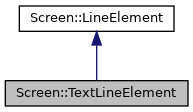
\includegraphics[width=217pt]{classScreen_1_1TextLineElement__inherit__graph}
\end{center}
\end{figure}


Collaboration diagram for Screen\+:\+:Text\+Line\+Element\+:\nopagebreak
\begin{figure}[H]
\begin{center}
\leavevmode
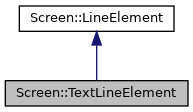
\includegraphics[width=217pt]{classScreen_1_1TextLineElement__coll__graph}
\end{center}
\end{figure}
\subsection*{Public Member Functions}
\begin{DoxyCompactItemize}
\item 
\mbox{\hyperlink{classScreen_1_1TextLineElement_ae0de60080a1c3f6c1be23448927e0717}{Text\+Line\+Element}} (std\+::string \mbox{\hyperlink{classScreen_1_1TextLineElement_ad2495931e2dd28b0d7cb5d8c761dedad}{text}}=\char`\"{}\char`\"{}, uint16\+\_\+t \mbox{\hyperlink{classScreen_1_1TextLineElement_ac4fa4d52ead8e4b38ba18c673875fae2}{color}}=0, int margin=0, bool \mbox{\hyperlink{classScreen_1_1LineElement_a0c5f4e33c2df1dce8e4e45b90dac1423}{align\+Right}}=false)
\begin{DoxyCompactList}\small\item\em \mbox{\hyperlink{classScreen_1_1TextLineElement}{Text\+Line\+Element}} constructor. \end{DoxyCompactList}\item 
\mbox{\hyperlink{classScreen_1_1TextLineElement_ae6f666d60594d487b9c43310c470ec59}{Text\+Line\+Element}} (std\+::string \mbox{\hyperlink{classScreen_1_1TextLineElement_ad2495931e2dd28b0d7cb5d8c761dedad}{text}}, uint16\+\_\+t \mbox{\hyperlink{classScreen_1_1TextLineElement_ac4fa4d52ead8e4b38ba18c673875fae2}{color}}, int \mbox{\hyperlink{classScreen_1_1LineElement_a9ed23f9510a11334af9be6f53965f7a6}{margin\+Left}}, int \mbox{\hyperlink{classScreen_1_1LineElement_a3a2077f01072be8e8fd0f4539b85beb0}{margin\+Right}}, bool \mbox{\hyperlink{classScreen_1_1LineElement_a0c5f4e33c2df1dce8e4e45b90dac1423}{align\+Right}}=false)
\begin{DoxyCompactList}\small\item\em \mbox{\hyperlink{classScreen_1_1TextLineElement}{Text\+Line\+Element}} constructor with different margins. \end{DoxyCompactList}\item 
int \mbox{\hyperlink{classScreen_1_1TextLineElement_abcd2e0700f84bb19d7a285345cd37871}{render\+Self}} (\mbox{\hyperlink{classDisplay}{Display}} $\ast$\mbox{\hyperlink{classScreen_aad713267725e8aa8a8def951a07de641}{display}}, int x, int y)
\begin{DoxyCompactList}\small\item\em Renders itself at position x, y to display. \end{DoxyCompactList}\end{DoxyCompactItemize}
\subsection*{Protected Attributes}
\begin{DoxyCompactItemize}
\item 
\mbox{\Hypertarget{classScreen_1_1TextLineElement_ad2495931e2dd28b0d7cb5d8c761dedad}\label{classScreen_1_1TextLineElement_ad2495931e2dd28b0d7cb5d8c761dedad}} 
std\+::string \mbox{\hyperlink{classScreen_1_1TextLineElement_ad2495931e2dd28b0d7cb5d8c761dedad}{text}}
\begin{DoxyCompactList}\small\item\em The text. \end{DoxyCompactList}\item 
\mbox{\Hypertarget{classScreen_1_1TextLineElement_ac4fa4d52ead8e4b38ba18c673875fae2}\label{classScreen_1_1TextLineElement_ac4fa4d52ead8e4b38ba18c673875fae2}} 
uint16\+\_\+t \mbox{\hyperlink{classScreen_1_1TextLineElement_ac4fa4d52ead8e4b38ba18c673875fae2}{color}}
\begin{DoxyCompactList}\small\item\em Color of the text. \end{DoxyCompactList}\end{DoxyCompactItemize}
\subsection*{Additional Inherited Members}


\subsection{Detailed Description}
Text. 

\subsection{Constructor \& Destructor Documentation}
\mbox{\Hypertarget{classScreen_1_1TextLineElement_ae0de60080a1c3f6c1be23448927e0717}\label{classScreen_1_1TextLineElement_ae0de60080a1c3f6c1be23448927e0717}} 
\index{Screen\+::\+Text\+Line\+Element@{Screen\+::\+Text\+Line\+Element}!Text\+Line\+Element@{Text\+Line\+Element}}
\index{Text\+Line\+Element@{Text\+Line\+Element}!Screen\+::\+Text\+Line\+Element@{Screen\+::\+Text\+Line\+Element}}
\subsubsection{\texorpdfstring{Text\+Line\+Element()}{TextLineElement()}\hspace{0.1cm}{\footnotesize\ttfamily [1/2]}}
{\footnotesize\ttfamily Screen\+::\+Text\+Line\+Element\+::\+Text\+Line\+Element (\begin{DoxyParamCaption}\item[{std\+::string}]{text = {\ttfamily \char`\"{}\char`\"{}},  }\item[{uint16\+\_\+t}]{color = {\ttfamily 0},  }\item[{int}]{margin = {\ttfamily 0},  }\item[{bool}]{align\+Right = {\ttfamily false} }\end{DoxyParamCaption})}



\mbox{\hyperlink{classScreen_1_1TextLineElement}{Text\+Line\+Element}} constructor. 


\begin{DoxyParams}[1]{Parameters}
\mbox{\tt in}  & {\em text} & \\
\hline
\mbox{\tt in}  & {\em color} & \\
\hline
\mbox{\tt in}  & {\em margin} & \\
\hline
\mbox{\tt in}  & {\em align\+Right} & \\
\hline
\end{DoxyParams}
\mbox{\Hypertarget{classScreen_1_1TextLineElement_ae6f666d60594d487b9c43310c470ec59}\label{classScreen_1_1TextLineElement_ae6f666d60594d487b9c43310c470ec59}} 
\index{Screen\+::\+Text\+Line\+Element@{Screen\+::\+Text\+Line\+Element}!Text\+Line\+Element@{Text\+Line\+Element}}
\index{Text\+Line\+Element@{Text\+Line\+Element}!Screen\+::\+Text\+Line\+Element@{Screen\+::\+Text\+Line\+Element}}
\subsubsection{\texorpdfstring{Text\+Line\+Element()}{TextLineElement()}\hspace{0.1cm}{\footnotesize\ttfamily [2/2]}}
{\footnotesize\ttfamily Screen\+::\+Text\+Line\+Element\+::\+Text\+Line\+Element (\begin{DoxyParamCaption}\item[{std\+::string}]{text,  }\item[{uint16\+\_\+t}]{color,  }\item[{int}]{margin\+Left,  }\item[{int}]{margin\+Right,  }\item[{bool}]{align\+Right = {\ttfamily false} }\end{DoxyParamCaption})}



\mbox{\hyperlink{classScreen_1_1TextLineElement}{Text\+Line\+Element}} constructor with different margins. 


\begin{DoxyParams}[1]{Parameters}
\mbox{\tt in}  & {\em text} & \\
\hline
\mbox{\tt in}  & {\em color} & \\
\hline
\mbox{\tt in}  & {\em margin\+Left} & \\
\hline
\mbox{\tt in}  & {\em margin\+Right} & \\
\hline
\mbox{\tt in}  & {\em align\+Right} & \\
\hline
\end{DoxyParams}


\subsection{Member Function Documentation}
\mbox{\Hypertarget{classScreen_1_1TextLineElement_abcd2e0700f84bb19d7a285345cd37871}\label{classScreen_1_1TextLineElement_abcd2e0700f84bb19d7a285345cd37871}} 
\index{Screen\+::\+Text\+Line\+Element@{Screen\+::\+Text\+Line\+Element}!render\+Self@{render\+Self}}
\index{render\+Self@{render\+Self}!Screen\+::\+Text\+Line\+Element@{Screen\+::\+Text\+Line\+Element}}
\subsubsection{\texorpdfstring{render\+Self()}{renderSelf()}}
{\footnotesize\ttfamily int Screen\+::\+Text\+Line\+Element\+::render\+Self (\begin{DoxyParamCaption}\item[{\mbox{\hyperlink{classDisplay}{Display}} $\ast$}]{display,  }\item[{int}]{x,  }\item[{int}]{y }\end{DoxyParamCaption})\hspace{0.3cm}{\ttfamily [virtual]}}



Renders itself at position x, y to display. 


\begin{DoxyParams}[1]{Parameters}
\mbox{\tt in}  & {\em display} & \mbox{\hyperlink{classDisplay}{Display}} to render to. \\
\hline
\mbox{\tt in}  & {\em x} & X position to render to. \\
\hline
\mbox{\tt in}  & {\em y} & Y position to render to. \\
\hline
\end{DoxyParams}
\begin{DoxyReturn}{Returns}
Number of pixels this elements takes. 
\end{DoxyReturn}


Implements \mbox{\hyperlink{classScreen_1_1LineElement_a667fbf6505fbed274ca9a3deac3fef9e}{Screen\+::\+Line\+Element}}.



The documentation for this class was generated from the following files\+:\begin{DoxyCompactItemize}
\item 
Display\+Utils/Screen.\+h\item 
Display\+Utils/Screen.\+cpp\end{DoxyCompactItemize}

\hypertarget{classUnitScreen}{}\section{Unit\+Screen Class Reference}
\label{classUnitScreen}\index{Unit\+Screen@{Unit\+Screen}}


Unit screen.  




{\ttfamily \#include $<$Unit\+Screen.\+h$>$}



Inheritance diagram for Unit\+Screen\+:\nopagebreak
\begin{figure}[H]
\begin{center}
\leavevmode
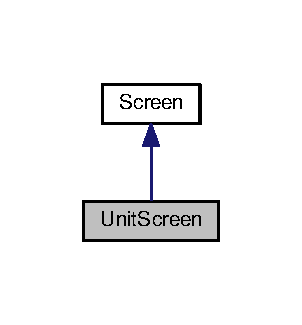
\includegraphics[width=145pt]{classUnitScreen__inherit__graph}
\end{center}
\end{figure}


Collaboration diagram for Unit\+Screen\+:\nopagebreak
\begin{figure}[H]
\begin{center}
\leavevmode
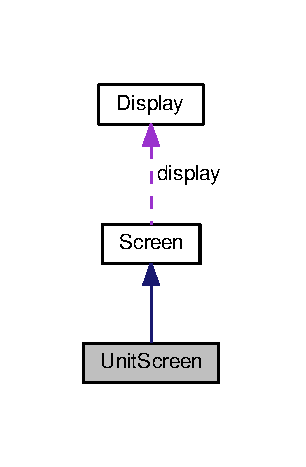
\includegraphics[width=147pt]{classUnitScreen__coll__graph}
\end{center}
\end{figure}
\subsection*{Public Member Functions}
\begin{DoxyCompactItemize}
\item 
\mbox{\Hypertarget{classUnitScreen_aec9e9c593e2c59025096fd01529c874b}\label{classUnitScreen_aec9e9c593e2c59025096fd01529c874b}} 
{\bfseries Unit\+Screen} (\mbox{\hyperlink{classDisplay}{Display}} $\ast$display, \mbox{\hyperlink{classLightUnit}{Light\+Unit}} \&unit)
\item 
\mbox{\Hypertarget{classUnitScreen_aa6baad6ccef6da111a44d763de359bb8}\label{classUnitScreen_aa6baad6ccef6da111a44d763de359bb8}} 
void \mbox{\hyperlink{classUnitScreen_aa6baad6ccef6da111a44d763de359bb8}{render\+Screen}} ()
\begin{DoxyCompactList}\small\item\em Renders this screen to display. \end{DoxyCompactList}\item 
\mbox{\Hypertarget{classUnitScreen_a4eea15b5c63c97c5a072b151cfa05e84}\label{classUnitScreen_a4eea15b5c63c97c5a072b151cfa05e84}} 
void \mbox{\hyperlink{classUnitScreen_a4eea15b5c63c97c5a072b151cfa05e84}{handle\+Knob\+Change}} (int8\+\_\+t R\+G\+B\+Delta\mbox{[}3\mbox{]})
\begin{DoxyCompactList}\small\item\em Handles knob changes. \end{DoxyCompactList}\item 
\mbox{\Hypertarget{classUnitScreen_a45956efc8827ebfdddaf83d7c44db135}\label{classUnitScreen_a45956efc8827ebfdddaf83d7c44db135}} 
void \mbox{\hyperlink{classUnitScreen_a45956efc8827ebfdddaf83d7c44db135}{handle\+Knob\+Press}} (bool R\+G\+B\+Pressed\mbox{[}3\mbox{]})
\begin{DoxyCompactList}\small\item\em Handles knob presses. \end{DoxyCompactList}\end{DoxyCompactItemize}
\subsection*{Additional Inherited Members}


\subsection{Detailed Description}
Unit screen. 

This screen renders info about selected unit and allows making changes to units light settings. 

The documentation for this class was generated from the following files\+:\begin{DoxyCompactItemize}
\item 
Display\+Utils/Unit\+Screen.\+h\item 
Display\+Utils/Unit\+Screen.\+cpp\end{DoxyCompactItemize}

%--- End generated contents ---

% Index
\backmatter
\newpage
\phantomsection
\clearemptydoublepage
\addcontentsline{toc}{chapter}{Index}
\printindex

\end{document}
